% Options for packages loaded elsewhere
% Options for packages loaded elsewhere
\PassOptionsToPackage{unicode}{hyperref}
\PassOptionsToPackage{hyphens}{url}
\PassOptionsToPackage{dvipsnames,svgnames,x11names}{xcolor}
%
\documentclass[
  french,
  9pt,
  a4paper,
]{article}
\usepackage{xcolor}
\usepackage[top = 3cm,bottom = 2.5cm,left = 2.5cm,right =
2.5cm]{geometry}
\usepackage{amsmath,amssymb}
\setcounter{secnumdepth}{3}
\usepackage{iftex}
\ifPDFTeX
  \usepackage[T1]{fontenc}
  \usepackage[utf8]{inputenc}
  \usepackage{textcomp} % provide euro and other symbols
\else % if luatex or xetex
  \usepackage{unicode-math} % this also loads fontspec
  \defaultfontfeatures{Scale=MatchLowercase}
  \defaultfontfeatures[\rmfamily]{Ligatures=TeX,Scale=1}
\fi
\usepackage{lmodern}
\ifPDFTeX\else
  % xetex/luatex font selection
\fi
% Use upquote if available, for straight quotes in verbatim environments
\IfFileExists{upquote.sty}{\usepackage{upquote}}{}
\IfFileExists{microtype.sty}{% use microtype if available
  \usepackage[]{microtype}
  \UseMicrotypeSet[protrusion]{basicmath} % disable protrusion for tt fonts
}{}
\usepackage{setspace}
\makeatletter
\@ifundefined{KOMAClassName}{% if non-KOMA class
  \IfFileExists{parskip.sty}{%
    \usepackage{parskip}
  }{% else
    \setlength{\parindent}{0pt}
    \setlength{\parskip}{6pt plus 2pt minus 1pt}}
}{% if KOMA class
  \KOMAoptions{parskip=half}}
\makeatother
% Make \paragraph and \subparagraph free-standing
\makeatletter
\ifx\paragraph\undefined\else
  \let\oldparagraph\paragraph
  \renewcommand{\paragraph}{
    \@ifstar
      \xxxParagraphStar
      \xxxParagraphNoStar
  }
  \newcommand{\xxxParagraphStar}[1]{\oldparagraph*{#1}\mbox{}}
  \newcommand{\xxxParagraphNoStar}[1]{\oldparagraph{#1}\mbox{}}
\fi
\ifx\subparagraph\undefined\else
  \let\oldsubparagraph\subparagraph
  \renewcommand{\subparagraph}{
    \@ifstar
      \xxxSubParagraphStar
      \xxxSubParagraphNoStar
  }
  \newcommand{\xxxSubParagraphStar}[1]{\oldsubparagraph*{#1}\mbox{}}
  \newcommand{\xxxSubParagraphNoStar}[1]{\oldsubparagraph{#1}\mbox{}}
\fi
\makeatother


\usepackage{longtable,booktabs,array}
\usepackage{calc} % for calculating minipage widths
% Correct order of tables after \paragraph or \subparagraph
\usepackage{etoolbox}
\makeatletter
\patchcmd\longtable{\par}{\if@noskipsec\mbox{}\fi\par}{}{}
\makeatother
% Allow footnotes in longtable head/foot
\IfFileExists{footnotehyper.sty}{\usepackage{footnotehyper}}{\usepackage{footnote}}
\makesavenoteenv{longtable}
\usepackage{graphicx}
\makeatletter
\newsavebox\pandoc@box
\newcommand*\pandocbounded[1]{% scales image to fit in text height/width
  \sbox\pandoc@box{#1}%
  \Gscale@div\@tempa{\textheight}{\dimexpr\ht\pandoc@box+\dp\pandoc@box\relax}%
  \Gscale@div\@tempb{\linewidth}{\wd\pandoc@box}%
  \ifdim\@tempb\p@<\@tempa\p@\let\@tempa\@tempb\fi% select the smaller of both
  \ifdim\@tempa\p@<\p@\scalebox{\@tempa}{\usebox\pandoc@box}%
  \else\usebox{\pandoc@box}%
  \fi%
}
% Set default figure placement to htbp
\def\fps@figure{htbp}
\makeatother


% definitions for citeproc citations
\NewDocumentCommand\citeproctext{}{}
\NewDocumentCommand\citeproc{mm}{%
  \begingroup\def\citeproctext{#2}\cite{#1}\endgroup}
\makeatletter
 % allow citations to break across lines
 \let\@cite@ofmt\@firstofone
 % avoid brackets around text for \cite:
 \def\@biblabel#1{}
 \def\@cite#1#2{{#1\if@tempswa , #2\fi}}
\makeatother
\newlength{\cslhangindent}
\setlength{\cslhangindent}{1.5em}
\newlength{\csllabelwidth}
\setlength{\csllabelwidth}{3em}
\newenvironment{CSLReferences}[2] % #1 hanging-indent, #2 entry-spacing
 {\begin{list}{}{%
  \setlength{\itemindent}{0pt}
  \setlength{\leftmargin}{0pt}
  \setlength{\parsep}{0pt}
  % turn on hanging indent if param 1 is 1
  \ifodd #1
   \setlength{\leftmargin}{\cslhangindent}
   \setlength{\itemindent}{-1\cslhangindent}
  \fi
  % set entry spacing
  \setlength{\itemsep}{#2\baselineskip}}}
 {\end{list}}
\usepackage{calc}
\newcommand{\CSLBlock}[1]{\hfill\break\parbox[t]{\linewidth}{\strut\ignorespaces#1\strut}}
\newcommand{\CSLLeftMargin}[1]{\parbox[t]{\csllabelwidth}{\strut#1\strut}}
\newcommand{\CSLRightInline}[1]{\parbox[t]{\linewidth - \csllabelwidth}{\strut#1\strut}}
\newcommand{\CSLIndent}[1]{\hspace{\cslhangindent}#1}

\ifLuaTeX
\usepackage[bidi=basic]{babel}
\else
\usepackage[bidi=default]{babel}
\fi
% get rid of language-specific shorthands (see #6817):
\let\LanguageShortHands\languageshorthands
\def\languageshorthands#1{}


\setlength{\emergencystretch}{3em} % prevent overfull lines

\providecommand{\tightlist}{%
  \setlength{\itemsep}{0pt}\setlength{\parskip}{0pt}}



 


\makeatletter
\@ifpackageloaded{tcolorbox}{}{\usepackage[skins,breakable]{tcolorbox}}
\@ifpackageloaded{fontawesome5}{}{\usepackage{fontawesome5}}
\definecolor{quarto-callout-color}{HTML}{909090}
\definecolor{quarto-callout-note-color}{HTML}{0758E5}
\definecolor{quarto-callout-important-color}{HTML}{CC1914}
\definecolor{quarto-callout-warning-color}{HTML}{EB9113}
\definecolor{quarto-callout-tip-color}{HTML}{00A047}
\definecolor{quarto-callout-caution-color}{HTML}{FC5300}
\definecolor{quarto-callout-color-frame}{HTML}{acacac}
\definecolor{quarto-callout-note-color-frame}{HTML}{4582ec}
\definecolor{quarto-callout-important-color-frame}{HTML}{d9534f}
\definecolor{quarto-callout-warning-color-frame}{HTML}{f0ad4e}
\definecolor{quarto-callout-tip-color-frame}{HTML}{02b875}
\definecolor{quarto-callout-caution-color-frame}{HTML}{fd7e14}
\makeatother
\makeatletter
\@ifpackageloaded{caption}{}{\usepackage{caption}}
\AtBeginDocument{%
\ifdefined\contentsname
  \renewcommand*\contentsname{Table des matières}
\else
  \newcommand\contentsname{Table des matières}
\fi
\ifdefined\listfigurename
  \renewcommand*\listfigurename{Graphiques}
\else
  \newcommand\listfigurename{Graphiques}
\fi
\ifdefined\listtablename
  \renewcommand*\listtablename{Tableaux}
\else
  \newcommand\listtablename{Tableaux}
\fi
\ifdefined\figurename
  \renewcommand*\figurename{Graphique}
\else
  \newcommand\figurename{Graphique}
\fi
\ifdefined\tablename
  \renewcommand*\tablename{Tableau}
\else
  \newcommand\tablename{Tableau}
\fi
}
\@ifpackageloaded{float}{}{\usepackage{float}}
\floatstyle{ruled}
\@ifundefined{c@chapter}{\newfloat{codelisting}{h}{lop}}{\newfloat{codelisting}{h}{lop}[chapter]}
\floatname{codelisting}{Listing}
\newcommand*\listoflistings{\listof{codelisting}{Liste des Listings}}
\makeatother
\makeatletter
\makeatother
\makeatletter
\@ifpackageloaded{caption}{}{\usepackage{caption}}
\@ifpackageloaded{subcaption}{}{\usepackage{subcaption}}
\makeatother
\usepackage{bookmark}
\IfFileExists{xurl.sty}{\usepackage{xurl}}{} % add URL line breaks if available
\urlstyle{same}
\hypersetup{
  pdftitle={Évolution de la pauvreté monétaire en France},
  pdfauthor={Pierre Madec},
  pdflang={fr},
  colorlinks=true,
  linkcolor={blue},
  filecolor={Maroon},
  citecolor={Blue},
  urlcolor={Blue},
  pdfcreator={LaTeX via pandoc}}

%%% title.tex we use to call other packages. Because this works
\usepackage{titlepic}
\usepackage{titling}
\usepackage{graphicx}
\usepackage{fontspec}
\usepackage{placeins}
\usepackage{graphbox}
\usepackage{tikz}
\usepackage{geometry}
\usepackage{xcolor}
\usepackage{amsmath}
\usepackage[some]{background}
\usepackage{lipsum}
\usepackage{caption}
\usepackage{datetime}
\usepackage{xstring}
\usepackage{blindtext}
\usepackage{scrlayer-scrpage}

\setmainfont{OpenSans}[
  UprightFont = {*-Regular},
  BoldFont = {*-Bold},
  BoldItalicFont = {*-BoldItalic},
  ItalicFont = {*-Italic},
  Path = {_extensions/ofce/wp/OpenSans/},
  Extension = {.ttf}
]
\setsansfont{OpenSans}[
  UprightFont = {*-Regular},
  BoldFont = {*-Bold},
  BoldItalicFont = {*-BoldItalic},
  ItalicFont = {*-Italic},
  Path = {_extensions/ofce/wp/OpenSans/},
  Extension = {.ttf}
]

\def\getYear#1{\StrLeft{#1}{4}}
\def\getMonth#1{\StrMid{#1}{6}{7}}
\def\getDay#1{\StrRight{#1}{2}}

\def\jolimois#1{\monthname{\getMonth{#1}}}

\definecolor{quarto-callout-color}{HTML}{eeeeee}
\definecolor{quarto-callout-tip-color}{HTML}{dddddd}
\definecolor{quarto-callout-tip-color-frame}{HTML}{eeeeee}

\clearpairofpagestyles

\KOMAoptions{headsepline=true}

\pagestyle{scrheadings}
\setkomafont{pageheadfoot}{\small}

\rehead{Document de travail n°2026-6}
\lohead{\includegraphics[height=0.25cm]{\_extensions/ofce/wp/ofce\_m.png}}

\lofoot*{\thepage}
\refoot*{\thepage}

\usepackage{etoolbox}
\AtBeginEnvironment{quote}{\par\singlespacing\small}

% Pour changer les notes de marge en texte de bas de page
\usepackage{marginnote}
\renewcommand{\marginnote}[1]{{#1}}

% spacing de la bibliographie
 \usepackage{calc}
  \renewenvironment{CSLReferences}[2] % #1 hanging-indent, #2 entry-spacing
    {\begin{list}{}{%
          \setlength{\itemindent}{0pt}
          \setlength{\leftmargin}{0pt}
          \setlength{\parsep}{0pt}
          % turn on hanging indent if param 1 is 1
          \ifodd #1
          \setlength{\leftmargin}{\cslhangindent}
          \setlength{\itemindent}{-1\cslhangindent}
          \fi
          % set entry spacing
          \setlength{\itemsep}{0.25\baselineskip}}} % hard-coded itemsep
    {\end{list}}

\begin{document}



\definecolor{ofcepbbleu}{RGB}{1, 97, 131}
\definecolor{ofcerouge}{RGB}{198, 45, 43}
\definecolor{scporouge}{RGB}{231, 0, 26}

\begin{titlepage}
  \backgroundsetup{
    scale=1,
    angle=0,
    opacity=1,
    contents={
  \begin{tikzpicture}[remember picture,overlay]
    \useasboundingbox (0,0) rectangle(\the\paperwidth,\the\paperheight);
      \node [anchor = center] at (-2.875-5.25,12.5) {\includegraphics[width=2.5cm]{\_extensions/ofce/wp/ofce\_m.png}};
      \node [anchor = center] at (-2.875-5.25,-12.75){
\includegraphics[width=2.5cm]{\_extensions/ofce/wp/sciencespo.png}};
      \node [anchor = east] at (8.5,-11.5){\textcolor{black}{Publié le : 25
mars 2026}};
      \node [anchor = east] at (8.5,-12){\textcolor{black}{Modifié le : 25
mars 2026}};
      \node [anchor = east] at (8.5,13-0.7){\textcolor{gray}{\Huge\textit{Working Paper}}};
      \draw [thick,black](-5.75,-13) -- (-5.75,13);
      \draw [color = white, fill=ofcepbbleu] (8.7,11.4) rectangle (10.45,13.15);
      \draw [color = white, fill=ofcepbbleu, very thick] (8.75-.5,11.25-.5) rectangle (8.75+.6,11.25+.6);
      \node [anchor = east] at (11-0.7,13-0.7){\textcolor{white}{\huge\textbf{6}}};
      \node [anchor = east] at (10-0.74,12-0.67){\textcolor{white}{\textbf{2026}}};
    \end{tikzpicture}
  }
}
\BgThispage

\hspace{4cm}
\begin{minipage}{12.5cm}
  \vspace{5cm}
  \begin{flushleft}
    \begin{spacing}{2.5}
      \textcolor{scporouge}{\Huge\textbf{\textsf{Évolution de la
pauvreté monétaire en France}}}
    \end{spacing}
      \vspace{5mm}
    \begin{spacing}{1.5}
      \textcolor{scporouge}{\large\textbf{\textsf{Dynamiques,
déterminants et reste à vivre\,: une analyse à partir des Enquêtes
Revenus Fiscaux et Sociaux (2005-2023)}}}
    \end{spacing}
    \vspace{5mm}
    \vspace{20mm}
  \end{flushleft}

      \textbf{Pierre Madec}
         ,
             OFCE, Sciences Po Paris
           
        \vspace{2mm}
    % by-author
 \end{minipage}

%%
%% deuxieme page
\newpage
\pagestyle{empty}
\raisebox{-22cm}{
    \begin{minipage}[b]{40em}
      \textcolor{scporouge}{
        \textbf{CONTACT}}{

          \vspace{0.2cm}
          \vspace{0.2cm}

        \textbf{OFCE}

        10 place de Catalogne

        75014 Paris, FRANCE

        Tel : +33 1 44 18 54 24

        \url{https://www.ofce.sciences-po.fr}
      }
    \end{minipage}
}
%%
%%
\newpage
%% troisieme page
\pagestyle{empty}
%%  \raisebox{3cm}{\begin{minipage}{\linewidth}
%%  \includegraphics[width=2cm]{\_extensions/ofce/wp/ofce\_m.png}
%%
%%  
\includegraphics[width=2cm]{\_extensions/ofce/wp/sciencespo.png}
%%  \end{minipage}}
%%

\LARGE\textbf{Évolution de la pauvreté monétaire en France}

\large\textbf{Dynamiques, déterminants et reste à vivre\,: une analyse à
partir des Enquêtes Revenus Fiscaux et Sociaux (2005-2023)}

\vspace{1cm}


\par\rule{\textwidth}{0.5pt}

Ce document de travail propose une analyse de la dynamique de la
pauvreté monétaire en France entre 2005 et 2023. Il examine les
déterminants de la hausse observée depuis 2018 en distinguant les effets
de seuil, de structure, de redistribution et de revenus primaires. Une
attention particulière est portée aux travailleurs pauvres et aux
ménages avec enfants. Au-delà de la pauvreté monétaire, l'analyse du «
reste à vivre » permet de tenir compte de la réalité des dépenses
contraintes.

\par\rule{\textwidth}{0.5pt}


\vspace{1cm}


version en ligne à https://pierremadec.github.io/Analyses\_pauvrete/


\vspace{1cm}

\begin{flushright}
   \linespread{1}\small{\textbf{Pierre
Madec}}, {\small{pierre.madec@ofce.sciences-po.fr}}\par
 % by-author
\end{flushright}
\end{titlepage}

%%% Define custom colors
% tip
\definecolor{quarto-callout-tip-color}{HTML}{000000}
\definecolor{quarto-callout-tip-color-frame}{HTML}{EEEEEE}

\vspace{2.5cm}

\renewcommand*\contentsname{Table des matières}
{
\hypersetup{linkcolor=}
\setcounter{tocdepth}{1}
\tableofcontents
}

\vspace{5cm}
\setstretch{1.25}
Malgré un système de protection sociale parmi les plus développés
d'Europe\,--- la France consacre plus de 31\,\% de son PIB aux dépenses
de protection sociale, contre 27\,\% en moyenne dans l'Union européenne
(Eurostat, 2023) ---, le taux de pauvreté a atteint 15,4\,\% en 2023,
soit près de 9,8~millions de personnes vivant sous le seuil de 60\,\% du
niveau de vie médian (INSEE, 2024). Ce niveau, le plus élevé observé
depuis le milieu des années 1990, interroge la capacité du modèle social
français à contenir la progression de la pauvreté dans un contexte de
forte inflation et de mutations du marché du travail. Au-delà de la
seule insuffisance de revenus monétaires, la pauvreté peut aussi
s'exprimer dans des défaillances d'accès aux services publics, aux
droits sociaux et aux modes de vie ordinaires (Madec et Pucci, 2025).

Ce document de travail propose une analyse en plusieurs temps à partir
des données individuelles de l'Enquête Revenus Fiscaux et Sociaux (ERFS)
de l'INSEE, couvrant la période 2005-2023. Après avoir dressé le constat
de la hausse de la pauvreté, en distinguant ses composantes avant et
après redistribution, nous nous attachons à identifier les déterminants
de cette hausse au moyen de deux décompositions complémentaires\,---
l'une macroéconomique, l'autre microéconomique de type Oaxaca-Blinder.
Enfin, nous estimerons le coût budgétaire théorique de l'éradication de
la pauvreté et proposerons d'aller au-delà de la pauvreté monétaire en
adoptant une approche par le « reste à vivre », qui intègre la réalité
des dépenses contraintes des ménages.

\section{Pauvreté monétaire en France\,: une dynamique
préoccupante}\label{pauvretuxe9-monuxe9taire-en-france-une-dynamique-pruxe9occupante}

La mesure de la pauvreté monétaire repose sur la comparaison du niveau
de vie des ménages à un seuil défini relativement à la distribution des
revenus. Ce choix d'un seuil relatif\,--- retenu par l'Union européenne
et l'INSEE\,--- traduit une conception sociale de la pauvreté\,: est
pauvre celui dont les ressources sont insuffisantes pour participer aux
modes de vie ordinaires de la société. Si cette approche présente
l'avantage de la simplicité et de la comparabilité internationale, elle
est par nature sensible aux mouvements de la médiane et se distingue
d'une mesure en termes absolus de pouvoir d'achat\footnote{Sur cette
  question de la construction de l'indicateur de pauvreté, voir
  notamment\,: Decerf, Benoit.~2022.~Absolute and Relative Poverty
  Measurement: A Survey.~Policy Research Working Paper;10008.~©~World
  Bank.~http://hdl.handle.net/10986/37325}. Nous distinguons ici trois
mesures complémentaires qui permettent d'éclairer en partie les
dynamiques à l'œuvre\,: le taux avant redistribution (calculé sur les
revenus primaires), le taux après redistribution au seuil courant de
60\,\% de la médiane, et le taux à seuil gelé (ici seuil de 2005
revalorisé par l'inflation) (Graphique~\ref{fig-taux-pauvrete}).

\begin{figure}

\caption{\label{fig-taux-pauvrete}Taux de pauvreté monétaire en France
métropolitaine (2005-2023)\,: avant redistribution, après redistribution
et à seuil gelé. Seuil à 60\,\% du revenu médian.}

\centering{

\pandocbounded{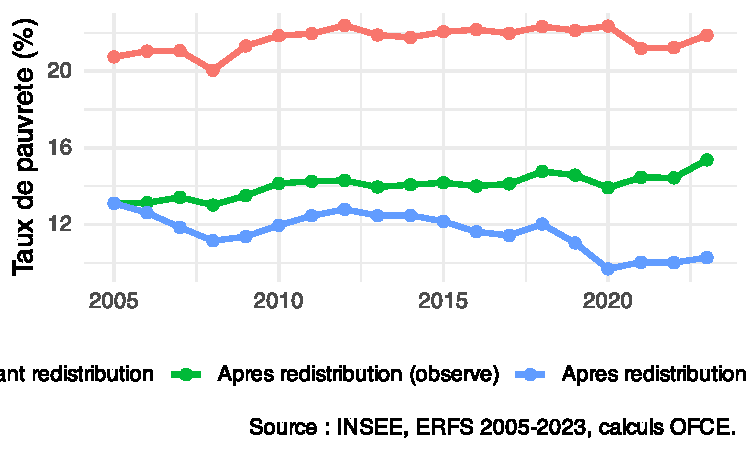
\includegraphics[keepaspectratio]{index_files/mediabag/index_files/figure-pdf/fig-taux-pauvrete-1.pdf}}

}

\end{figure}%

Le graphique révèle un écart significatif entre le taux « officiel »
(seuil relatif courant) et le taux à seuil gelé. Cet écart illustre
l'enjeu fondamental du choix entre une mesure en termes absolus de
pouvoir d'achat et une mesure relative à la distribution des revenus. Le
débat est ancien, mais les arguments en faveur du seuil relatif restent
convaincants. Comme le souligne De Schutter (2021), rapporteur spécial
de l'ONU sur l'extrême pauvreté, les plus modestes vivent dans les mêmes
espaces sociaux et géographiques que le reste de la population\,---
notamment dans des villes où le coût de la vie, en particulier du
logement, augmente à mesure que la société s'enrichit. L'exclusion
sociale provient précisément de l'écart entre ce que la moyenne de la
population peut se permettre et ce qui reste accessible aux plus
modestes.

Cependant, le seuil relatif possède une faiblesse majeure qui apparaît
lors des chocs macroéconomiques\,: il peut masquer une détérioration
réelle des conditions de vie derrière une amélioration statistique, dès
lors que les revenus du bas de la distribution baissent moins que ceux
de la médiane. C'est ce que nous verrons avec la crise financière de
2008-2009.

Le \emph{taux de pauvreté calculé sur les revenus primaires} (avant
redistribution) oscille entre 20\,\% et 22\,\% sur l'ensemble de la
période, sans tendance claire. Cette stabilité apparente masque des
mouvements de sens contraire\,: la hausse du taux d'emploi est compensée
par la progression des emplois précaires et du temps partiel subi
(DARES, 2022~; Ponthieux, 2006).

La crise financière de 2008-2009 produit un effet contre-intuitif\,: le
taux avant redistribution baisse temporairement avant de remonter en
2009 et en 2010. Ce mouvement résulte d'une mécanique bien comprise\,:
l'impact de la crise a été d'abord plus violent sur le revenu médian
(affecté par les pertes d'emplois et les baisses de rémunération des
salariés) que sur les revenus des plus pauvres, qui étaient déjà en
partie en dehors du marché du travail. Le seuil de pauvreté a donc
baissé plus vite que les revenus des pauvres, créant une baisse
mécanique du taux\,--- sans que la situation réelle des plus modestes se
soit améliorée. C'est la limitation majeure d'un seuil relatif\,: il
peut masquer une détérioration réelle des conditions de vie derrière une
amélioration statistique. Ce phénomène se reproduit en 2020 lors du choc
du COVID-19.

Le \emph{taux de pauvreté après redistribution} connaît une trajectoire
plus heurtée. Après avoir baissé entre 2007 et 2008, il remonte de 2009
à 2011 dans le sillage de la crise financière, révélant un rattrapage
progressif du seuil. Une période de relative stabilité s'étend de 2012 à
2017. En 2018 et 2019, sous l'effet à la fois de la baisse des aides au
logement et des soutiens au revenu médian (prime d'activité, taxe
d'habitation,\,\ldots), le taux de pauvreté augmente fortement.
Exception faite de la crise Covid dont les effets sont signalés plus
haut, le taux de pauvreté réaugmente fortement après la crise sanitaire
pour culminer à 15,4\,\% en 2023 (Lelièvre et Pucci, 2025).

Le \emph{taux à seuil gelé} --- qui neutralise l'effet de la progression
de la médiane\,--- suit quant à lui globalement une tendance baissière,
passant de 13,1\,\% en 2005 à 10,3\,\% en 2023. Ce décalage illustre que
la hausse du taux de pauvreté «\,officiel\,» est en grande partie le
reflet de la mesure relative. En termes de pouvoir d'achat absolu, la
situation des ménages les plus modestes s'est moins dégradée que celle
du ménage médian\,: pendant les crises, les revenus primaires du bas de
la distribution baissent moins que ceux de la médiane, ce qui produit
mécaniquement une baisse du taux de pauvreté (par baisse du seuil) sans
amélioration réelle. La crise de 2008-2009 en offre l'illustration la
plus nette, illustrant la limite majeure du seuil relatif\footnote{Voir
  notamment O. De Schutter (2021), \emph{Extreme poverty and human
  rights}, Report of the Special Rapporteur, United Nations A/HRC/47/36,
  juin 2021, §§ 14-18. Voir aussi l'intervention disponible sur\,:
  \url{https://www.youtube.com/watch?v=DG5PkgFraBc}}.

L'écart entre le taux avant et après redistribution\,--- qui mesure
l'efficacité du système socio-fiscal à réduire la pauvreté--- s'est
réduit au fil du temps, passant de 7,6~points en 2005 à 6,5~points en
2023. Le système redistributif « sort » de moins en moins de ménages de
la pauvreté\footnote{Voir notamment\,: P. Madec,
  «\,\href{https://www.ofce.sciences-po.fr/blog2024/fr/2025/20251125_PIM/20251125_PIM.fr.pdf}{Lutte
  contre la pauvreté: le décrochage français}\,», Blog de l'OFCE, 2024.}.
Plusieurs mécanismes contribuent à cette érosion\,: le décrochage des
minima sociaux par rapport au seuil de pauvreté, le non-recours aux
prestations\,--- estimé à environ 30-35\,\% des ayants droit pour le RSA
(DREES, 2019) --- et les effets de certaines réformes socio-fiscales qui
ont réduit les transferts en direction des ménages modestes.

Cette érosion de l'efficacité redistributive trouve une explication
directe dans l'évolution comparée des trois principaux repères de
revenus\,: le RSA socle, le SMIC net et le revenu médian. La lecture en
base 100 met en évidence les écarts de dynamique entre les trois séries,
tandis que la lecture en euros courants rappelle les niveaux absolus\,:
en 2023, le SMIC net mensuel atteint environ 1\,430\,€, le RSA socle
pour une personne seule 635\,€, et le revenu médian mensuel par unité de
consommation environ 2\,000\,€.

Graphique 2\,--- Évolution comparée du RSA socle, du SMIC net à temps
plein et du revenu médian.

\subsection{Base 100 (2005)}

\pandocbounded{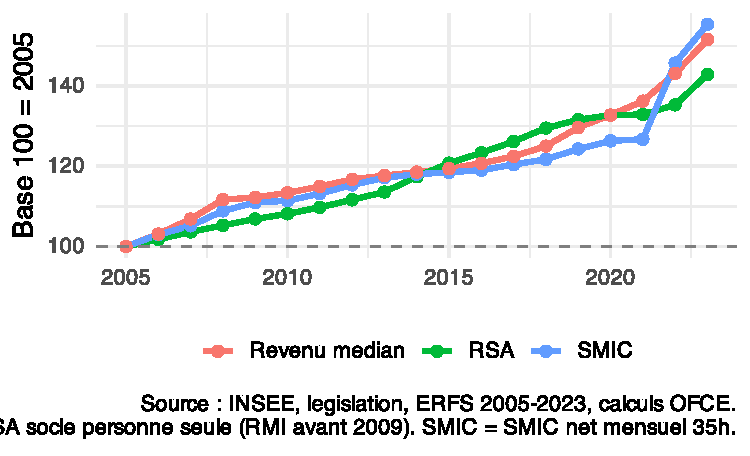
\includegraphics[keepaspectratio]{index_files/mediabag/index_files/figure-pdf/unnamed-chunk-1-1.pdf}}

\subsection{Euros courants}

\pandocbounded{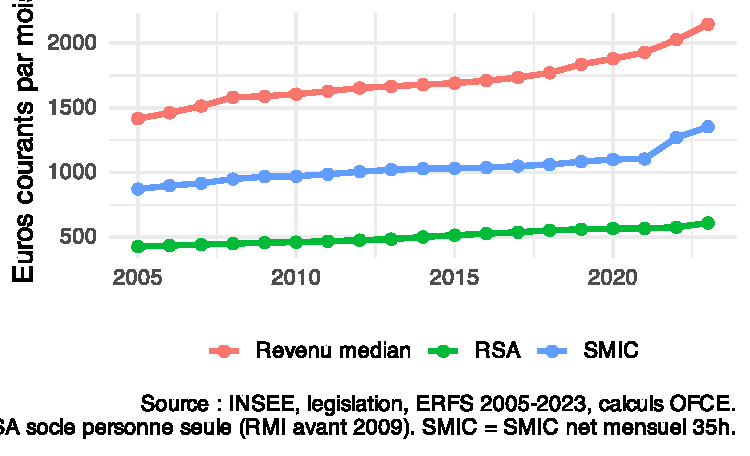
\includegraphics[keepaspectratio]{index_files/mediabag/index_files/figure-pdf/unnamed-chunk-2-1.pdf}}

\subsection{Écarts cumulés}

\pandocbounded{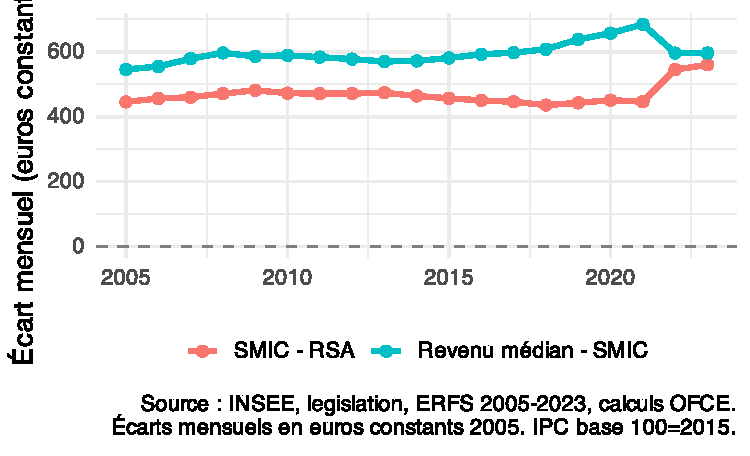
\includegraphics[keepaspectratio]{index_files/mediabag/index_files/figure-pdf/unnamed-chunk-3-1.pdf}}

Jusqu'en 2014, les trois séries évoluent de concert, avec une
progression d'environ 15 à 20\,\% en neuf ans. Le plan de revalorisation
du RSA de 10\,\% sur cinq ans, engagé en 2013 dans le cadre du Plan
pluriannuel de lutte contre la pauvreté (IGAS, 2017), permet brièvement
au RSA de rejoindre le rythme de la médiane. Cependant, cette dynamique
s'essouffle dès la fin des revalorisations exceptionnelles, et le RSA
retrouve un rythme de progression inférieur à celui du SMIC et de la
médiane.

La période 2020-2023 est marquée par un décrochage sans précédent. Le
SMIC\footnote{Le SMIC bénéficie de revalorisations automatiques gérées
  par le Comité supérieur de l'emploi des salaires et de l'ajustement
  professionnel, qui interviennent dès que l'inflation atteint ou
  dépasse 2\,\%. Des coups de pouce ponctuels (notamment en 2019 et
  2022) ont amplifié cette dynamique.}, bénéficiant de revalorisations
automatiques indexées sur l'inflation, a augmenté de 55\,\% par rapport
à 2005. Le revenu médian\footnote{Le revenu médian est calculé à partir
  de l'ensemble des revenus (salaires, revenus du capital, loyers
  fictifs, prestations), dont environ 40\,\% provient des salaires. Son
  évolution reflète à la fois la progression des rémunérations du
  travail et celle du capital.} a, lui, progressé de 50\,\%. Le
RSA\footnote{Le RSA a connu plusieurs revalorisations ponctuelles (coups
  de pouce) depuis 2013, mais sans mécanisme d'indexation automatique
  comparable à celui du SMIC. Les revalorisations interviennent
  généralement au 1er avril et selon des décisions budgétaires
  annuelles, d'où un décalage structurel par rapport aux autres revenus.},
revalorisé avec retard et selon des modalités moins protectrices, n'a,
lui, progressé que de 43\,\%. Ce décrochage de plus de 10~points par
rapport au SMIC traduit un éloignement croissant des allocataires par
rapport au seuil de pauvreté, contribuant à la fois à la hausse de
l'intensité de la pauvreté et à l'augmentation du coût de son
éradication. Le troisième onglet du graphique
(\textbf{?@fig-rsa-smic-ecarts}) met en évidence cette divergence en
montrant l'écart croissant entre le SMIC et le RSA depuis 2014, et entre
le revenu médian et le SMIC depuis 2018.

\begin{tcolorbox}[enhanced jigsaw, leftrule=.75mm, breakable, toptitle=1mm, toprule=.15mm, title={Encadré 1\,--- Pauvreté monétaire et logement\,: le biais des
prestations logement}, opacityback=0, arc=.35mm, opacitybacktitle=0.6, colback=white, coltitle=black, colframe=quarto-callout-note-color-frame, left=2mm, colbacktitle=quarto-callout-note-color!10!white, bottomtitle=1mm, titlerule=0mm, rightrule=.15mm, bottomrule=.15mm]

Le taux de pauvreté monétaire standard est calculé à partir du revenu
disponible, qui intègre les allocations logement (APL, ALS, ALF) en
ressources. Or, ces prestations ont vocation à couvrir une dépense\,---
le loyer\,--- qui n'est pas déduite du revenu dans le calcul du niveau
de vie. Cette asymétrie de traitement conduit à une sous-estimation du
taux de pauvreté des locataires, dont le revenu « disponible » inclut
des ressources fléchées et non librement arbitrables. Symétriquement,
les propriétaires ne perçoivent pas d'APL mais bénéficient d'un avantage
en nature\,--- les « loyers fictifs »\,--- qui n'est pas non plus
comptabilisé dans le revenu disponible (microéconomique) standard. Ce
traitement asymétrique est discuté de longue date par les statisticiens.
L'INSEE publie d'ailleurs des indicateurs complémentaires intégrant les
loyers fictifs, qui modifient sensiblement le diagnostic sur la pauvreté
des personnes âgées, majoritairement propriétaires. Cette question sera
reprise dans la dernière section consacrée au reste à vivre, qui intègre
directement les dépenses de logement (voir section 5).

Pour illustrer le biais concrètement\,: considérons un salarié vivant
seul avec un revenu identique. S'il est locataire, ses APL sont
comptabilisées dans son revenu disponible\,--- son niveau de vie
apparent est donc artificiellement gonflé par rapport à celui d'un
propriétaire percevant le même salaire mais sans aide au logement. Le
locataire apparaît ainsi « plus riche » en termes de niveau de vie,
alors qu'une fraction de ses ressources est directement absorbée par le
loyer.

Pour mesurer l'ampleur de ce biais, on peut recalculer le taux de
pauvreté en retirant les prestations logement du revenu disponible et en
distinguant propriétaires et locataires
(Graphique~\ref{fig-taux-occ-apl}).

\begin{figure}[H]

\caption{\label{fig-taux-occ-apl}Taux de pauvreté des propriétaires et
des locataires, avec et sans prise en compte des APL dans le calcul du
revenu disponible (2005-2023). Seuil à 60\,\% de la médiane.}

\centering{

\pandocbounded{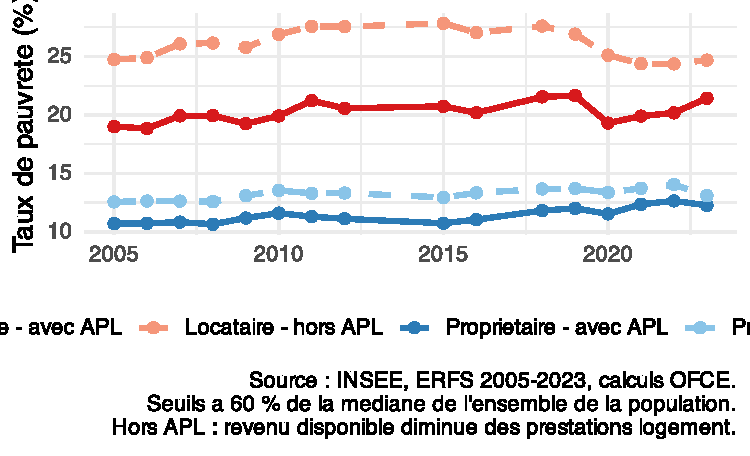
\includegraphics[keepaspectratio]{index_files/mediabag/index_files/figure-pdf/fig-taux-occ-apl-1.pdf}}

}

\end{figure}%

L'écart entre locataires et propriétaires est considérable et
persistant\,: les locataires affichent un taux de pauvreté environ trois
fois supérieur à celui des propriétaires. Le retrait des allocations
logement du revenu disponible accroît mécaniquement le taux de pauvreté
des locataires, confirmant le rôle de « correction statistique » joué
par les APL. Pour les propriétaires, l'écart entre les deux mesures est
logiquement faible puisqu'ils perçoivent peu d'aides au logement. Ce
différentiel reflète à la fois un effet de sélection\,--- les ménages
modestes sont plus souvent locataires\,--- et l'impact du coût du
logement sur le reste à vivre effectif. La progression du taux de
pauvreté des locataires sur la période récente est nettement plus
marquée que celle des propriétaires, confirmant la vulnérabilité
particulière de cette population face aux chocs de prix.

\end{tcolorbox}

\section{Les déterminants de la hausse de la
pauvreté}\label{les-duxe9terminants-de-la-hausse-de-la-pauvretuxe9}

La hausse de la pauvreté monétaire depuis 2018 ne résulte pas d'un
facteur unique mais de la conjonction de plusieurs mécanismes. Pour les
identifier et les hiérarchiser, nous mobilisons deux approches
complémentaires\,: une décomposition séquentielle, qui isole les effets
de seuil, de structure, de redistribution et de revenus primaires\,; et
une décomposition microéconomique de type Oaxaca-Blinder, qui permet de
distinguer les effets de composition (changement des caractéristiques de
la population) des effets de coefficients (changement du risque de
pauvreté associé à chaque caractéristique).

La décomposition de la variation du taux de pauvreté par rapport à 2005
fait ressortir la prédominance de l'effet seuil dans la hausse observée
(Graphique~\ref{fig-decomposition}).

\begin{figure}

\caption{\label{fig-decomposition}Décomposition de la variation du taux
de pauvreté par rapport à 2005 (en points de pourcentage)\,: effets de
seuil, de structure, de redistribution et de revenus primaires.}

\centering{

\pandocbounded{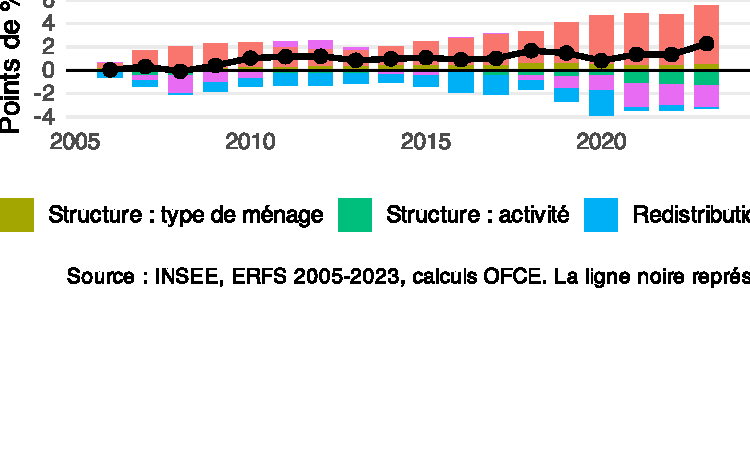
\includegraphics[keepaspectratio]{index_files/mediabag/index_files/figure-pdf/fig-decomposition-1.pdf}}

}

\end{figure}%

L'effet seuil constitue le principal facteur d'augmentation apparente de
la pauvreté. Il contribue à hauteur de +2~points entre 2006 et 2013,
puis s'amplifie nettement à partir de 2018 pour atteindre +5~points en
2022-2023. Cette accélération résulte directement de la poussée
inflationniste\,: les revenus nominaux\,--- et donc la médiane\,--- ont
progressé rapidement, entraînant le seuil de pauvreté à la hausse plus
vite que les bas revenus. Ce résultat souligne le caractère
intrinsèquement relatif de la mesure de la pauvreté monétaire,
c'est-à-dire du décrochage des plus modestes relativement aux standards
de consommation de la société.

\begin{tcolorbox}[enhanced jigsaw, leftrule=.75mm, breakable, toptitle=1mm, toprule=.15mm, title={Encadré 2\,--- Méthode de décomposition séquentielle}, opacityback=0, arc=.35mm, opacitybacktitle=0.6, colback=white, coltitle=black, colframe=quarto-callout-note-color-frame, left=2mm, colbacktitle=quarto-callout-note-color!10!white, bottomtitle=1mm, titlerule=0mm, rightrule=.15mm, bottomrule=.15mm]

La variation du taux de pauvreté entre une année \emph{t} et l'année de
référence (2005) est décomposée en quatre effets au moyen de simulations
contrefactuelles successives\,:

\begin{enumerate}
\def\labelenumi{\arabic{enumi}.}
\tightlist
\item
  Effet seuil\,: on substitue au seuil de pauvreté courant un seuil «
  gelé » (seuil de 2005 revalorisé par l'IPC). La différence entre le
  taux observé et le taux à seuil gelé mesure la contribution de la
  hausse relative du seuil.
\item
  Effet structure\,: à seuil gelé, on repondère la population pour lui
  imposer la structure démographique de 2005 (type de ménage × statut
  d'activité). L'écart entre le taux à seuil gelé et le taux à seuil
  gelé et structure constante isole la contribution des changements de
  composition.
\item
  Effet redistribution\,: à seuil gelé et structure constante, on
  neutralise les transferts socio-fiscaux pour isoler l'évolution de
  leur efficacité.
\item
  Effet revenus primaires\,: le résidu mesure l'évolution des revenus
  avant redistribution, à seuil gelé et structure constante.
\end{enumerate}

La somme des quatre effets est, par construction, égale à la variation
totale du taux de pauvreté. L'ordre de décomposition peut influencer
marginalement les contributions estimées\,; la séquence retenue ici
privilégie l'identification de l'effet seuil, considéré comme le plus
exogène.

\end{tcolorbox}

Excepté sur la période 2011-2013 où les revenus primaires ont contribué
à l'augmentation de la pauvreté ce qui illustre les points évoqués plus
haut, l'effet des revenus primaires est négatif sur presque toute la
période, atteignant -2 à -3~points en fin de période. À seuil gelé et
structure constante, les revenus du travail et du capital des ménages
modestes se sont donc globalement améliorés, sous l'effet conjugué de la
hausse du taux d'emploi et des revalorisations du SMIC.

Les effets de structure demeurent modestes. On relève toutefois un léger
effet positif lié à la hausse de la part des personnes seules et des
familles monoparentales\footnote{De par leur composition (un revenu mais
  plus d'une unité de consommation) et leurs caractéristiques, ces
  familles ont un risque de pauvreté monétaire plus important ((Bonnet C
  et Solaz, 2022)).} --- dont la proportion dans la population française
a progressé de 16\,\% à près de 26\,\% des familles avec enfants entre
1990 et 2020 (INSEE, 2023a) ---, ainsi qu'un épisode ponctuel en
2020-2021 lié aux modifications de la structure d'activité induites par
la crise sanitaire.

L'effet redistribution confirme l'érosion progressive de l'efficacité du
système socio-fiscal à réduire les inégalités dans le bas de la
distribution (Madec, 2025), cohérente avec le décrochage du RSA
documenté dans la section précédente.

\subsection{Emploi et pauvreté\,: le paradoxe des travailleurs
pauvres}\label{emploi-et-pauvretuxe9-le-paradoxe-des-travailleurs-pauvres}

La période récente se caractérise par une amélioration significative du
marché du travail\,--- recul du chômage, hausse du taux d'emploi\,---
qui ne s'est pas traduite par une baisse de la pauvreté monétaire. Ce
découplage apparent invite à examiner de plus près le lien entre statut
d'activité et risque de pauvreté (Graphique~\ref{fig-taux-activite}).

\begin{figure}

\caption{\label{fig-taux-activite}Taux de pauvreté monétaire selon le
statut d'activité de la personne de référence (2010-2023). Seuil commun
à 60\,\% de la médiane.}

\centering{

\pandocbounded{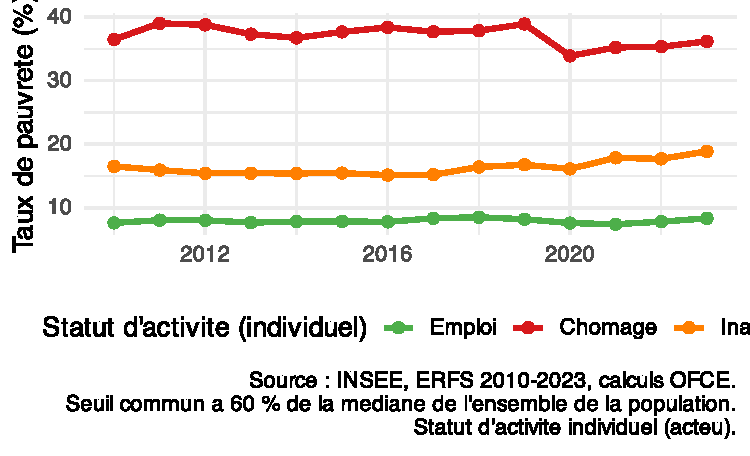
\includegraphics[keepaspectratio]{index_files/mediabag/index_files/figure-pdf/fig-taux-activite-1.pdf}}

}

\end{figure}%

Le taux de pauvreté des ménages dont la personne de référence\footnote{La
  personne de référence du ménage est déterminée en tenant compte de
  l'activité, du fait d'avoir un conjoint, du fait d'avoir un enfant et
  de l'âge. Parmi les personnes permanentes du ménage, la personne de
  référence est, si elle est unique, la personne active ayant un
  conjoint, sinon la personne active la plus âgée ayant un conjoint. À
  défaut de personne active ayant un conjoint, la personne la plus âgée
  ayant un conjoint. À défaut de personne ayant un conjoint, la personne
  active la plus âgée ayant un enfant. À défaut de personne active ayant
  un enfant, la personne active la plus âgée. À défaut de personne
  active, la personne ayant un enfant la plus âgée. À défaut de personne
  ayant un enfant, la personne la plus âgée.} est en emploi demeure
nettement inférieur à celui des chômeurs et des inactifs. Sa progression
au cours de la période récente s'explique par la combinaison de la
hausse du seuil de pauvreté (effet mécanique de la mesure relative) et
de la multiplication des emplois à faible rémunération, à temps partiel
subi ou à durée limitée (DARES, 2022~; Ponthieux, 2006). L'emploi
protège de moins en moins de la pauvreté, en particulier pour les
ménages mono-actifs et les familles monoparentales (par définition au
mieux mono-active). Ce phénomène, bien documenté à l'échelle européenne
(Eurofound, 2017), s'observe avec une intensité particulière en France,
où le recours aux contrats courts s'est accentué depuis le milieu des
années 2000.

Au-delà des taux, la composition de la population pauvre selon le statut
d'activité révèle des dynamiques contrastées entre groupes
(Graphique~\ref{fig-compo-pauvres}).

\begin{figure}

\caption{\label{fig-compo-pauvres}Composition de la population des
ménages pauvres selon le statut d'activité de la personne de référence
(2010-2023), en\,\% du total des ménages pauvres.}

\centering{

\pandocbounded{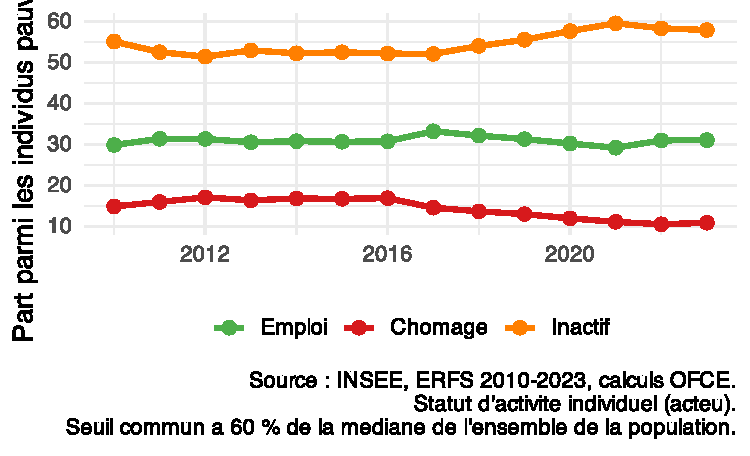
\includegraphics[keepaspectratio]{index_files/mediabag/index_files/figure-pdf/fig-compo-pauvres-1.pdf}}

}

\end{figure}%

Trois tendances se dégagent. La part des ménages inactifs dans la
population pauvre est en hausse marquée sur l'ensemble de la période.
Cette progression reflète deux mécanismes distincts\,: d'un côté,
l'accumulation de situations de non-emploi durable\,; de l'autre, une
précarisation progressive des retraités. Dans un régime de pauvreté
relative, les pensions\,--- indexées sur l'inflation\,--- décrochent
mécaniquement par rapport au seuil dès lors que le niveau de vie médian
croît plus vite que les prix, ce qui gonfle la part des retraités
pauvres indépendamment de toute dégradation de leur pouvoir d'achat
absolu. Concomitamment, la part des chômeurs parmi les ménages pauvres
diminue sur la période. Cette évolution reflète principalement la baisse
tendancielle du taux de chômage depuis 2015. Le Comité scientifique du
CNLE (Pucci, Lelièvre et Auzuret, 2025) montre que cette baisse a
concerné y compris les chômeurs de longue durée\,--- le taux de chômage
de longue durée a reculé de 2,3~points entre 2015 et 2022\,--- et que
les sorties du chômage vers l'emploi ont largement concerné ces profils,
réfutant l'idée que seuls les individus les plus proches du marché du
travail auraient bénéficié de la reprise. Enfin, si la part des actifs
occupés parmi les ménages pauvres a progressé depuis 2010\,--- portée
par la croissance de l'emploi peu qualifié et à temps partiel\,---, elle
se situe en 2023 à un niveau quasi identique à celui de 2017, suggérant
une relative stabilisation du phénomène de \emph{travail pauvre} en
proportion de la pauvreté totale.

Ces évolutions agrégées masquent toutefois des transformations
structurelles au sein des ménages pauvres. Deux dynamiques
démographiques majeures modifient la composition de la pauvreté\,: d'une
part, la polarisation de l'emploi au sein des couples, avec une
progression de la bi-activité chez les ménages aisés tandis que les
couples pauvres restent plus souvent mono-actifs, ce qui accentue
l'écart de niveau de vie entre les deux groupes\,; d'autre part,
l'augmentation continue des familles monoparentales (Haut Conseil de la
famille, de l'enfance et de l'âge (HCFEA), 2024a), qui cumulent revenu
unique et charges familiales élevées. Ces deux tendances renforcent le
rôle du nombre de personnes à charge et du statut d'activité du conjoint
comme déterminants majeurs de la pauvreté\,--- un mécanisme que les
décompositions microéconomiques présentées plus loin permettront de
quantifier précisément.

La notion de « travailleur pauvre » repose sur une tension
méthodologique fondamentale\,: la pauvreté se mesure au niveau du ménage
(le niveau de vie est calculé en rapportant le revenu disponible du
ménage au nombre d'unités de consommation), tandis que l'emploi est une
caractéristique individuelle. Un travailleur pauvre n'est donc pas
nécessairement un travailleur mal payé\,: c'est un individu en emploi
dont le ménage est pauvre (Ponthieux, 2006, 2009). Deux profils types se
dégagent\,: d'une part, des travailleurs à emploi stable mais dont les
charges familiales sont élevées (familles nombreuses mono-actives)\,;
d'autre part, des travailleurs précaires (temps partiel subi, CDD,
intérim) dont la faible rémunération individuelle ne permet pas au
ménage de franchir le seuil. Cette tension entre unité de mesure (le
ménage) et unité d'analyse (l'individu) confère à la pauvreté laborieuse
un caractère profondément genré\,: les femmes, surreprésentées dans
l'emploi à temps partiel et dans les familles monoparentales, sont
structurellement plus exposées au risque de pauvreté que les hommes,
alors même que la mesure au niveau du ménage tend à masquer cette
inégalité en supposant un partage égalitaire des ressources au sein du
couple (Périvier, 2016).

Pour comprendre les mécanismes à l'œuvre, on examine successivement les
ressources des ménages travailleurs pauvres\,--- revenus primaires et
prestations sociales\,--- et les conditions de travail de leur personne
de référence, telles qu'elles ressortent de la base individus de l'ERFS.

Le Graphique~\ref{fig-tp-decomp} décompose le niveau de vie moyen des
travailleurs pauvres en revenu primaire et en prestations sociales
ventilées par catégorie, en euros courants par UC et par mois. Il permet
d'apprécier le poids respectif de chaque composante et son évolution sur
la période.

\begin{figure}

\caption{\label{fig-tp-decomp}Décomposition du niveau de vie moyen des
travailleurs pauvres (2010-2023). En euros courants par unité de
consommation et par mois. Les flèches rouges indiquent l'écart entre le
niveau de vie moyen et le seuil de pauvreté.}

\centering{

\pandocbounded{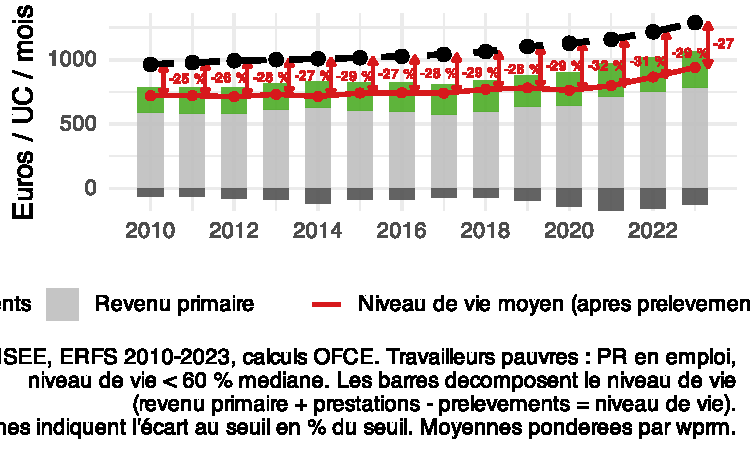
\includegraphics[keepaspectratio]{index_files/mediabag/index_files/figure-pdf/fig-tp-decomp-1.pdf}}

}

\end{figure}%

Le revenu primaire constitue de loin la composante dominante du niveau
de vie des travailleurs pauvres et croît en valeur nominale sur la
période, sous l'effet de la hausse du SMIC et de la progression des
salaires bas. Les prestations sociales s'y ajoutent en complément, sans
en modifier l'ordre de grandeur. Leur composition a toutefois évolué\,:
la prime d'activité, créée en 2016 par fusion du RSA activité et de la
PPE, a progressé en importance relative. Parallèlement, les aides au
logement (APL) ont vu leur rôle s'éroder depuis la réforme de 2017 (gel
des barèmes, puis contemporisation), et le RSA socle s'est dévalué en
termes réels. Ces évolutions de politique sociale ont eu des effets
contrastés sur le niveau de vie des travailleurs pauvres et expliquent
en partie pourquoi le pouvoir d'achat de ce groupe stagne malgré la
progression nominale de leurs revenus d'activité. Le graphique met en
évidence que malgré ces évolutions, l'écart entre le niveau de vie des
travailleurs pauvres et le seuil de pauvreté s'est creusé, s'aggravant
de manière particulière après 2020.

La comparaison de la composition familiale entre travailleurs pauvres et
travailleurs non pauvres met en lumière des différences structurelles
marquées (Graphique~\ref{fig-tp-typmen}). Chez les travailleurs non
pauvres, les couples avec enfant(s) dominent largement (environ
45-50\,\%), suivis des couples sans enfant (environ 25\,\%). À
l'inverse, chez les travailleurs pauvres, si les couples avec enfant(s)
restent la catégorie modale (environ 40\,\%), les familles
monoparentales et les personnes seules représentent ensemble près de la
moitié des ménages. Cette surreprésentation des configurations à revenu
unique est un trait distinctif de la pauvreté laborieuse\,: sans second
apporteur de ressources, un emploi mal rémunéré ou à temps partiel
suffit à faire basculer le ménage sous le seuil de pauvreté. La
remarquable stabilité de cette composition au fil du temps contraste
avec la dégradation observée des niveaux de vie, suggérant que c'est
moins la structure des ménages qui a changé que les conditions
économiques auxquelles ils font face.

\begin{figure}

\caption{\label{fig-tp-typmen}Composition des ménages de travailleurs
selon le type de ménage (2010-2023)\,: travailleurs pauvres vs
travailleurs non pauvres, en\,\% du groupe.}

\centering{

\pandocbounded{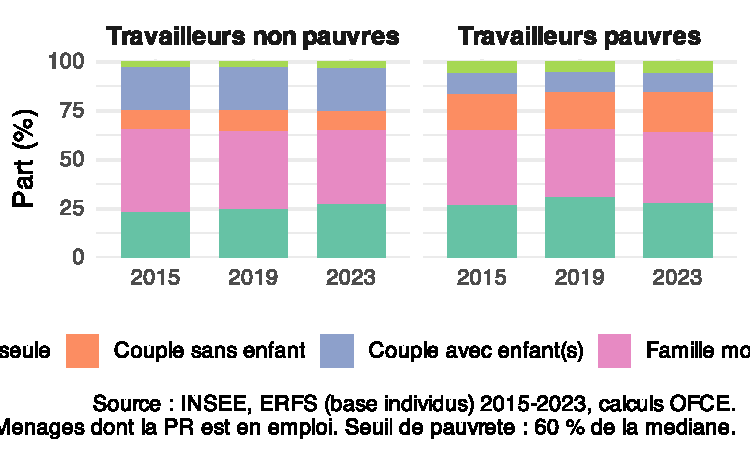
\includegraphics[keepaspectratio]{index_files/mediabag/index_files/figure-pdf/fig-tp-typmen-1.pdf}}

}

\end{figure}%

Les données de la base individus ERFS permettent d'aller au-delà du seul
statut emploi/chômage et d'examiner les conditions contractuelles de la
personne de référence du ménage. Le contraste entre travailleurs pauvres
et travailleurs non pauvres est saisissant
(Graphique~\ref{fig-tp-contrat})\,: les travailleurs pauvres sont plus
fréquemment titulaires de contrats à durée déterminée ou de missions
d'intérim, alors que le CDI domine très largement chez les travailleurs
non pauvres. Cette structure contractuelle plus précaire contribue au
niveau inférieur de rémunération\,--- les CDD et l'intérim impliquent
des périodes de non-emploi plus fréquentes\,--- et limite l'accès aux
dispositifs de formation et d'avancement (DARES, 2022~; Ponthieux,
2006). Pour autant, la précarité contractuelle n'est ni la seule ni la
principale explication de la pauvreté laborieuse\,: une part
substantielle des travailleurs pauvres est en CDI, mais la faiblesse de
leur rémunération rapportée au nombre de personnes à charge dans le
ménage suffit à les placer sous le seuil. La section suivante sur la
structure socioprofessionnelle illustre cette articulation entre
conditions d'emploi individuelles et configuration familiale.

\begin{figure}

\caption{\label{fig-tp-contrat}Type de contrat des actifs occupés
(personne de référence du ménage)\,: travailleurs pauvres vs
travailleurs non pauvres (2015, 2019, 2023), en\,\% des actifs occupés
hors contrats non renseignés.}

\centering{

\pandocbounded{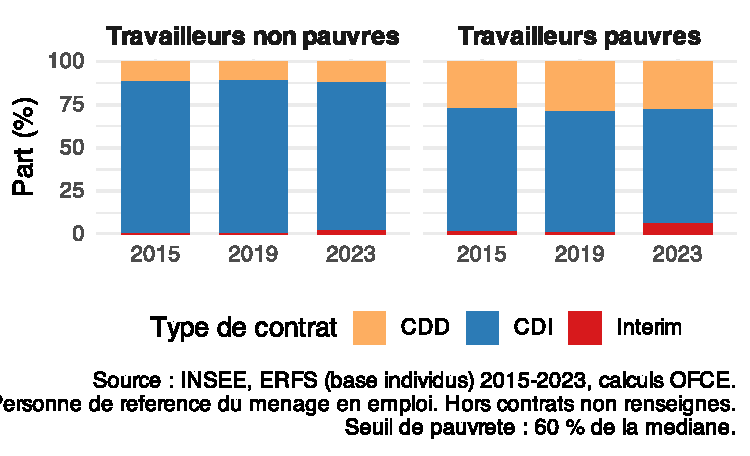
\includegraphics[keepaspectratio]{index_files/mediabag/index_files/figure-pdf/fig-tp-contrat-1.pdf}}

}

\end{figure}%

La structure socioprofessionnelle des travailleurs pauvres diffère
profondément de celle des travailleurs non pauvres
(Graphique~\ref{fig-tp-pcs}). Les ouvriers et employés peu qualifiés y
sont fortement surreprésentés, tandis que les cadres et professions
intermédiaires sont quasi absents. Pour autant, cette surreprésentation
ne se réduit pas à un effet de précarité contractuelle. Un ouvrier en
CDI au SMIC à temps plein, dont la conjointe est inactive et qui a trois
enfants à charge, se trouve mécaniquement sous le seuil de pauvreté\,---
non pas en raison de la qualité de son emploi, mais du rapport entre sa
rémunération individuelle et le nombre d'unités de consommation de son
ménage. C'est ici que la tension entre mesure individuelle de l'emploi
et mesure ménage de la pauvreté, soulignée par Périvier (2016) et
Ponthieux (2009), prend tout son sens\,: le nombre de personnes à charge
et le statut d'activité du conjoint sont au moins aussi déterminants que
le type de contrat ou le niveau de qualification pour expliquer le
basculement dans la pauvreté laborieuse. Les décompositions
Oaxaca-Blinder présentées plus loin confirmeront ce diagnostic en
montrant que le type de ménage et l'activité du conjoint dominent
largement les effets de coefficients.

\begin{figure}

\caption{\label{fig-tp-pcs}Catégorie socioprofessionnelle des actifs
occupés (personne de référence du ménage)\,: travailleurs pauvres vs
travailleurs non pauvres (2015, 2019, 2023), en\,\% du groupe.}

\centering{

\pandocbounded{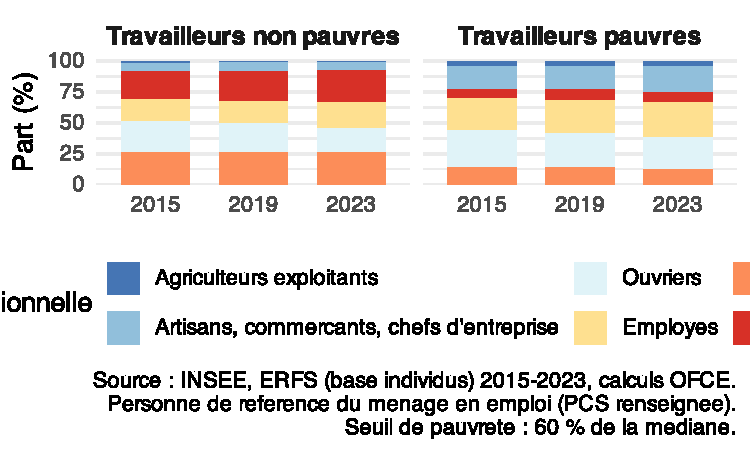
\includegraphics[keepaspectratio]{index_files/mediabag/index_files/figure-pdf/fig-tp-pcs-1.pdf}}

}

\end{figure}%

\subsection{Décomposition microéconomique de type
Oaxaca-Blinder}\label{duxe9composition-microuxe9conomique-de-type-oaxaca-blinder}

En résumé, la hausse de la pauvreté entre 2017 et 2023 tient davantage à
une aggravation du risque de pauvreté pour des profils donnés qu'à un
changement de composition de la population. Parmi les facteurs
explicatifs, l'activité du conjoint joue un rôle central\,: la
polarisation croissante de l'emploi dans les couples\,--- davantage de
biactifs \emph{et} davantage de mono-actifs\,--- domine à la fois les
effets de composition et de coefficients. Les familles monoparentales et
l'activité individuelle contribuent également, mais dans une moindre
mesure ((Haut Conseil de la famille, de l'enfance et de l'âge (HCFEA),
2024a)). Les résultats suivants permettent de quantifier précisément ces
contributions.

Pour compléter la décomposition séquentielle, qui raisonne sur des
agrégats, on mobilise une approche microéconomique permettant
d'identifier les caractéristiques individuelles qui contribuent le plus
à la variation du taux de pauvreté. La décomposition de Oaxaca (1973),
initialement développée pour l'analyse des écarts de salaires entre
groupes, est ici adaptée à l'étude de la pauvreté via l'extension logit
proposée par Fairlie (2005). Un modèle logit pondéré est estimé
séparément pour 2017 et 2023, la variable dépendante étant l'indicatrice
de pauvreté monétaire (seuil à 60\,\% de la médiane). Les variables
explicatives retenues sont\,: l'âge (8 classes), le sexe, le statut
d'immigration, le diplôme (5 niveaux), le type de ménage, l'activité
individuelle et l'activité du conjoint.

La variation du taux de pauvreté entre les deux dates est décomposée en
un effet de composition (ou « dotations »)\,--- la population a changé
de caractéristiques observables\,--- et un effet de coefficients (ou «
rendements »)\,--- le risque de pauvreté associé à chaque
caractéristique a évolué. Cette distinction permet de répondre à une
question centrale\,: la hausse de la pauvreté tient-elle davantage à un
changement de la structure de la population (davantage de profils
vulnérables) ou à une aggravation du risque de pauvreté pour des profils
donnés\,?

La décomposition par variable fait apparaître des contributions très
hétérogènes selon la dimension considérée
(Graphique~\ref{fig-oaxaca-variables}).

\begin{figure}

\caption{\label{fig-oaxaca-variables}Décomposition Oaxaca-Blinder de la
variation du taux de pauvreté entre 2017 et 2023, par variable\,: effets
de composition et de coefficients (en points de pourcentage).}

\centering{

\pandocbounded{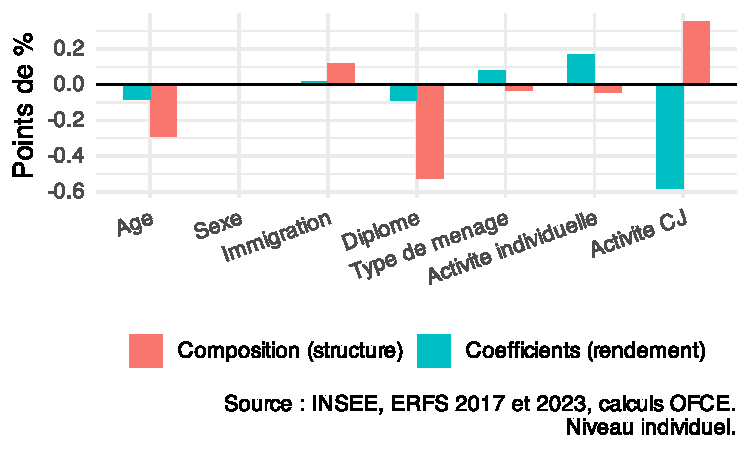
\includegraphics[keepaspectratio]{index_files/mediabag/index_files/figure-pdf/fig-oaxaca-variables-1.pdf}}

}

\end{figure}%

La décomposition par variable (Graphique~\ref{fig-oaxaca-variables})
fait ressortir trois résultats principaux. Du côté de la composition, le
diplôme constitue le principal facteur protecteur\,: l'élévation
générale du niveau d'éducation réduit la pauvreté d'environ -0,5~point.
Le vieillissement de la population contribue également à la baisse
(-0,25~point). En sens inverse, l'activité du conjoint (+0,3~point),
l'activité individuelle (+0,2~point) et l'immigration (+0,1~point)
poussent la pauvreté à la hausse. Du côté des coefficients, l'activité
du conjoint domine très largement avec une contribution de
-0,6~point\,--- le rendement protecteur de la bi-activité s'est
nettement renforcé entre 2017 et 2023. L'activité individuelle
(+0,17~point) et le type de ménage (+0,08~point) contribuent plus
modestement à la hausse. Les autres variables (âge, diplôme, sexe,
immigration) ont des effets de coefficients négligeables. Les résultats
détaillés par modalité (\emph{infra}) permettent de préciser ces
mécanismes.

\begin{tcolorbox}[enhanced jigsaw, leftrule=.75mm, breakable, toptitle=1mm, toprule=.15mm, title={Encadré 3\,--- Formalisation de la décomposition Oaxaca-Blinder}, opacityback=0, arc=.35mm, opacitybacktitle=0.6, colback=white, coltitle=black, colframe=quarto-callout-note-color-frame, left=2mm, colbacktitle=quarto-callout-note-color!10!white, bottomtitle=1mm, titlerule=0mm, rightrule=.15mm, bottomrule=.15mm]

Soit \(\bar{P}_t\) le taux de pauvreté observé à la date \(t\) et
\(\hat{P}_t = \frac{1}{N_t}\sum_i F(X_{i,t} \hat\beta_t)\) le taux
prédit par le modèle logit, où \(F\) désigne la fonction logistique,
\(X_t\) la matrice des caractéristiques observables et \(\hat\beta_t\)
le vecteur des coefficients estimés. On définit le contrefactuel
\(\hat{P}_{t_1|t_0} = \frac{1}{N_{t_1}}\sum_i F(X_{i,t_1} \hat\beta_{t_0})\)
--- le taux de pauvreté qui prévaudrait si la population de
\(t_1 = 2023\) faisait face aux coefficients de \(t_0 = 2017\). La
variation observée se décompose (Fairlie, 2005) en\,:

\[\bar{P}_{t_1} - \bar{P}_{t_0} = \underbrace{\hat{P}_{t_1|t_0} - \hat{P}_{t_0}}_{\text{Effet composition}} + \underbrace{(\bar{P}_{t_1} - \bar{P}_{t_0}) - (\hat{P}_{t_1|t_0} - \hat{P}_{t_0})}_{\text{Effet coefficients (résidu)}}\]

L'effet composition est évalué en appliquant les coefficients de l'année
de référence (\(\hat\beta_{t_0}\)) aux caractéristiques de l'année
finale\,--- il mesure ce qu'aurait été la variation du taux si seule la
structure de la population avait changé. L'effet coefficients est obtenu
par résidu. Dans un modèle linéaire, la décomposition OB classique se
décline en trois termes\,--- composition, coefficients et interaction
\((X_{t_1} - X_{t_0})(\beta_{t_1} - \beta_{t_0})\) --- qui capte l'effet
simultané des changements de caractéristiques et de rendements. Dans le
cadre non-linéaire du logit, cette séparation exacte n'est plus
possible. L'approche \emph{twofold} de Fairlie (2005) contourne cette
difficulté\,: le contrefactuel est construit avec les coefficients de la
période de référence (\(\hat\beta_{t_0}\)) et les caractéristiques de la
période finale (\(X_{t_1}\)), de sorte que le terme d'interaction est
absorbé dans l'effet coefficients. Ce dernier capture donc à la fois le
changement pur des rendements et l'interaction entre les évolutions
simultanées des caractéristiques et des rendements.

Les contributions par variable sont calculées à partir des effets
marginaux moyens (AME). Pour chaque modalité \(j\) d'une variable
catégorielle, la contribution par la composition est approximée par\,:

\[\Delta_j^{\text{compo}} \approx (\bar{p}_{j,t_1} - \bar{p}_{j,t_0}) \times \beta_j^{\text{dev}} \times \overline{F'(X\beta_{t_0})}\]

et la contribution par les coefficients par\,:

\[\Delta_j^{\text{coef}} \approx \bar{p}_{j,t_1} \times (\beta_{j,t_1}^{\text{dev}} - \beta_{j,t_0}^{\text{dev}}) \times \overline{F'(X\beta_{t_1})}\]

où \(\bar{p}_{j,t}\) désigne la proportion pondérée de la modalité \(j\)
à la date \(t\), \(\beta_j^{\text{dev}}\) le coefficient de déviation
associé et \(\overline{F'}\) l'effet marginal moyen. Cette linéarisation
permet une interprétation par modalité, mais ne somme pas exactement à
l'effet total en raison de la non-linéarité du modèle logit.

Normalisation de Yun (2005). La décomposition détaillée de l'effet des
coefficients par modalité d'une variable catégorielle est sujette à un
problème d'identification bien connu (Oaxaca et Ransom, 1999) : dans un
codage en indicatrices classique (\emph{treatment contrasts}), les
contributions individuelles dépendent du choix de la modalité de
référence omise. Pour lever cette indétermination, nous adoptons la
normalisation proposée par Yun (2005), qui repose sur des contrastes de
déviation (\emph{sum-to-zero constraints}). En pratique, le modèle logit
est estimé avec le codage standard (treatment contrasts), puis les
coefficients sont convertis en contrastes de déviation par la
transformation \(\beta_j^{\text{dev}} = \hat\beta_j - \bar{\hat\beta}\),
où \(\bar{\hat\beta} = \frac{1}{K}\sum_{k=1}^K \hat\beta_k\) et
\(\hat\beta_1 = 0\) pour la modalité de référence. Chaque coefficient
\(\beta_j^{\text{dev}}\) mesure alors l'écart de la modalité \(j\) à la
moyenne générale de la variable, et non l'écart à une modalité de
référence arbitraire. La contrainte \(\sum_j \beta_j^{\text{dev}} = 0\)
est satisfaite par construction. Cette reparamétrisation rend les
contributions détaillées invariantes au choix de la catégorie de
référence, tout en préservant l'identité de la décomposition globale.

\end{tcolorbox}

L'examen des vingt premières contributions par la composition permet de
préciser les mécanismes à l'œuvre (Graphique~\ref{fig-oaxaca-compo}).

\begin{figure}

\caption{\label{fig-oaxaca-compo}Décomposition Oaxaca-Blinder\,: vingt
principales contributions par la composition (en points de
pourcentage).}

\centering{

\pandocbounded{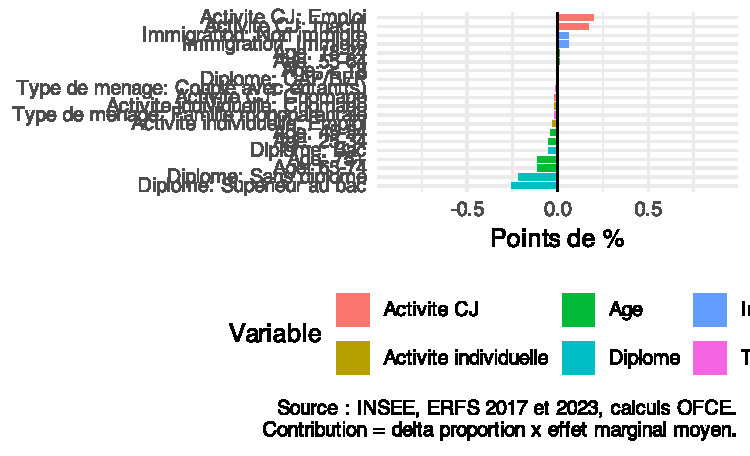
\includegraphics[keepaspectratio]{index_files/mediabag/index_files/figure-pdf/fig-oaxaca-compo-1.pdf}}

}

\end{figure}%

L'élévation générale du niveau d'éducation constitue le premier facteur
protecteur par la composition\,: la progression des diplômés du
supérieur au bac (-0,35~point) et la diminution des sans diplôme
(-0,25~point) réduisent conjointement la pauvreté d'environ 0,6~point.
Le vieillissement de la population, via la hausse de la part des
65-74~ans et des 75~ans et plus, exerce un effet protecteur
complémentaire (environ -0,2~point au total), lié au minimum vieillesse
et aux pensions de retraite. En sens inverse, l'activité du conjoint
domine les contributions positives\,: la hausse de la proportion de
conjoints en emploi (+0,15~point) et, symétriquement, de conjoints
inactifs (+0,12~point) traduit la polarisation croissante de l'emploi
dans les couples\,--- davantage de biactifs \emph{et} davantage de
mono-actifs. L'immigration contribue également, modestement, à la hausse
par la composition.

Du côté des coefficients, la hiérarchie des contributions met en
évidence le rôle central de l'activité du conjoint et, dans une moindre
mesure, du type de ménage (Graphique~\ref{fig-oaxaca-coeff}).

\begin{figure}

\caption{\label{fig-oaxaca-coeff}Décomposition Oaxaca-Blinder\,: vingt
principales contributions par les coefficients (en points de
pourcentage).}

\centering{

\pandocbounded{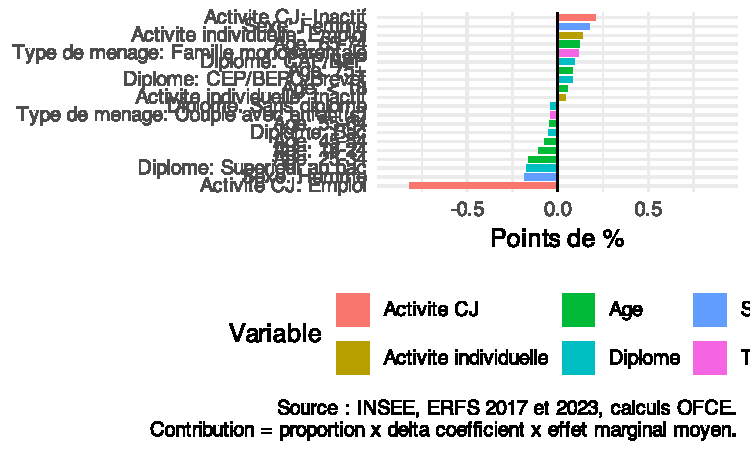
\includegraphics[keepaspectratio]{index_files/mediabag/index_files/figure-pdf/fig-oaxaca-coeff-1.pdf}}

}

\end{figure}%

Le résultat le plus saillant est la contribution de l'activité du
conjoint\,: l'emploi du conjoint réduit la pauvreté de -0,8~point (le
rendement protecteur de la bi-activité s'est renforcé), tandis que
l'inactivité du conjoint contribue à +0,3~point. Cet écart croissant
entre conjoints actifs et inactifs confirme que la bi-activité est
devenue une condition de plus en plus nécessaire pour échapper à la
pauvreté. La modalité « famille monoparentale » contribue à environ
+0,15~point par les coefficients\,: le surrisque de pauvreté associé à
la monoparentalité s'est accru entre 2017 et 2023. L'effet « Sexe\,:
Femme » (+0,1~point) signale une légère aggravation spécifique du risque
féminin, cohérente avec l'analyse de Périvier (2016). Du côté
protecteur, le diplôme supérieur au bac (-0,3~point) et l'emploi du
conjoint confirment que capital humain et bi-activité constituent les
principaux remparts contre la pauvreté.

\begin{tcolorbox}[enhanced jigsaw, leftrule=.75mm, breakable, toptitle=1mm, toprule=.15mm, title={Encadré 4\,--- Familles monoparentales\,: revenus primaires ou
prestations sociales\,?}, opacityback=0, arc=.35mm, opacitybacktitle=0.6, colback=white, coltitle=black, colframe=quarto-callout-note-color-frame, left=2mm, colbacktitle=quarto-callout-note-color!10!white, bottomtitle=1mm, titlerule=0mm, rightrule=.15mm, bottomrule=.15mm]

Bien que la contribution des familles monoparentales par les
coefficients soit modeste dans la décomposition d'ensemble
(+0,15~point), elle signale une aggravation du surrisque de pauvreté
associé à cette configuration familiale. Pour en comprendre les
mécanismes, on décompose l'évolution de leur niveau de vie en deux
composantes\,: le revenu primaire (avant redistribution) et les
prestations sociales reçues, elles-mêmes ventilées en quatre postes
(Graphique~\ref{fig-mono-decomp}).

\begin{figure}[H]

\caption{\label{fig-mono-decomp}Décomposition du niveau de vie moyen des
familles monoparentales (2005-2023)\,: revenu primaire, prestations
sociales par catégorie, niveau de vie total et seuil de pauvreté. En
euros courants par unité de consommation et par mois.}

\centering{

\pandocbounded{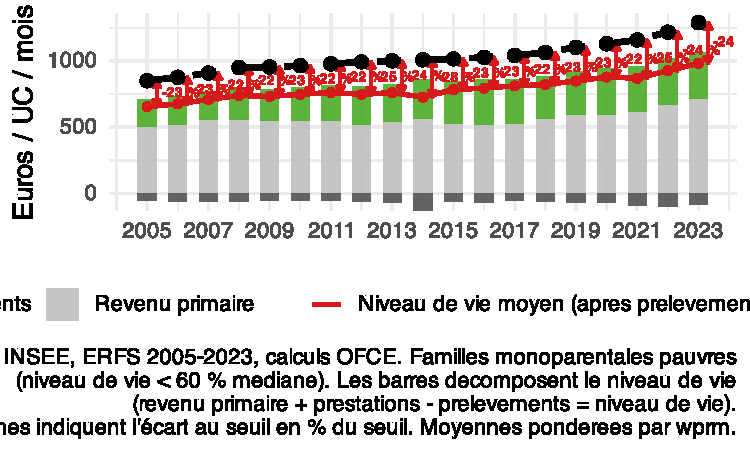
\includegraphics[keepaspectratio]{index_files/mediabag/index_files/figure-pdf/fig-mono-decomp-1.pdf}}

}

\end{figure}%

Trois enseignements se dégagent de cette décomposition.

Premier enseignement. Le niveau de vie avant redistribution des familles
monoparentales a progressé sur la période, porté par les revalorisations
du SMIC et la hausse du taux d'emploi des femmes seules avec enfants.
Cependant, cette progression est restée en deçà de celle du niveau de
vie médian\,--- et donc du seuil de pauvreté. La mesure relative de la
pauvreté capte précisément ce décrochage relatif.

Deuxième enseignement. La contribution des prestations sociales au
niveau de vie des familles monoparentales ne s'est pas accrue
proportionnellement à la hausse du seuil. Trois mécanismes se
cumulent\,:

\begin{itemize}
\tightlist
\item
  Le RSA a décroché d'environ 10~points par rapport au SMIC sur la
  période 2014-2023, réduisant la protection offerte aux familles
  monoparentales allocataires\,--- qui représentent près d'un tiers des
  bénéficiaires du RSA.
\item
  Les aides au logement (APL) ont été partiellement gelées\,: la réforme
  de 2017 (contemporisation, puis gel du barème) a réduit leur valeur
  réelle, particulièrement pénalisante pour les familles monoparentales,
  majoritairement locataires du parc privé.
\item
  Les prestations familiales ont été soumises à des mesures d'économies.
  L'érosion réelle du complément familial et de l'ASF (allocation de
  soutien familial, spécifique aux familles monoparentales), notamment
  n'ont pas suivi la progression du seuil ((Haut Conseil de la famille,
  de l'enfance et de l'âge (HCFEA), 2024b)).
\end{itemize}

Troisième enseignement. La conjonction de ces deux dynamiques\,---
revenu primaire progressant moins vite que la médiane et transferts
insuffisamment revalorisés\,--- a engendré un écart croissant entre le
niveau de vie des familles monoparentales et le seuil de pauvreté. La
dégradation du coefficient « famille monoparentale » dans la
décomposition Oaxaca-Blinder tient ainsi davantage à l'incapacité du
système socio-fiscal à compenser la hausse relative du seuil de pauvreté
qu'à une détérioration de leur situation sur le marché du travail. Ce
diagnostic plaide pour un ciblage prioritaire de la revalorisation des
minima sociaux et des aides au logement sur cette catégorie de ménages
(IGAS, 2017).

La décomposition par statut d'activité confirme que l'inactivité
constitue le principal facteur de vulnérabilité
(Graphique~\ref{fig-mono-activite})\,: les familles monoparentales dont
la personne de référence est inactive affichent un taux de pauvreté
nettement supérieur à celles en emploi ou au chômage. Sur la période
2017-2023, c'est avant tout la dégradation de la situation des
monoparentales en emploi\,--- dont le taux de pauvreté a progressé
malgré l'amélioration générale du marché du travail\,--- qui contribue à
la hausse du coefficient dans la décomposition Oaxaca-Blinder.

\begin{figure}[H]

\caption{\label{fig-mono-activite}Taux de pauvreté des familles
monoparentales selon le statut d'activité de la personne de référence
(2005-2023). Seuil à 60\,\% de la médiane.}

\centering{

\pandocbounded{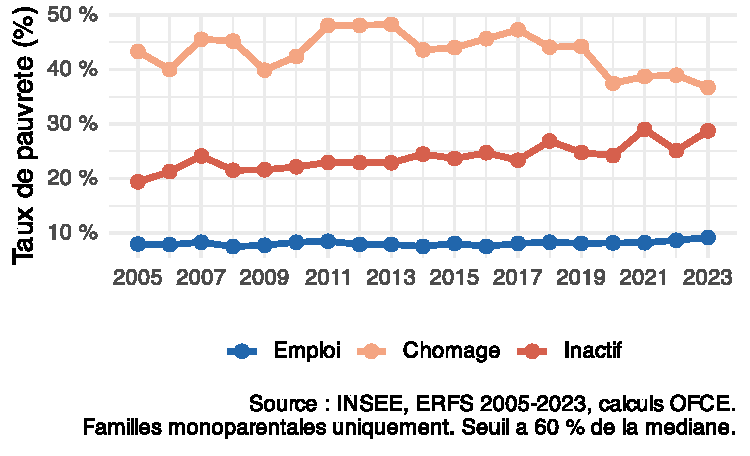
\includegraphics[keepaspectratio]{index_files/mediabag/index_files/figure-pdf/fig-mono-activite-1.pdf}}

}

\end{figure}%

\end{tcolorbox}

En revenant à la décomposition Oaxaca-Blinder menée sur l'ensemble des
ménages, la lecture d'ensemble des contributions par les coefficients
confirme le diagnostic central de cette analyse\,: c'est l'activité du
conjoint qui détermine le plus l'évolution du risque de pauvreté, bien
davantage que les caractéristiques individuelles d'emploi ou de
qualification. La bi-activité dans le couple est devenue une condition
de plus en plus nécessaire pour échapper à la pauvreté, tandis que la
monoparentalité, l'inactivité et le faible niveau de diplôme aggravent
le risque à la marge. Cette primauté de la dimension ménage dans
l'explication de la pauvreté renvoie à la tension structurelle entre
mesure individuelle de l'emploi et mesure ménage du niveau de vie,
soulignée par Périvier (2016) et Ponthieux (2009).

\section{Le coût budgétaire de l'éradication de la
pauvreté}\label{le-couxfbt-budguxe9taire-de-luxe9radication-de-la-pauvretuxe9}

Le déficit de revenu agrégé de l'ensemble des ménages pauvres par
rapport au seuil\,--- le \emph{poverty gap} --- fournit un plancher
théorique du montant nécessaire pour éliminer la pauvreté monétaire.
L'évolution de ce montant dans le temps permet de mesurer le coût
croissant de l'inaction.

\begin{tcolorbox}[enhanced jigsaw, leftrule=.75mm, breakable, toptitle=1mm, toprule=.15mm, title={Encadré 5\,--- Estimation du \emph{poverty gap}}, opacityback=0, arc=.35mm, opacitybacktitle=0.6, colback=white, coltitle=black, colframe=quarto-callout-note-color-frame, left=2mm, colbacktitle=quarto-callout-note-color!10!white, bottomtitle=1mm, titlerule=0mm, rightrule=.15mm, bottomrule=.15mm]

Le \emph{poverty gap} (écart de pauvreté agrégé) mesure la somme des
déficits de revenu de l'ensemble des ménages pauvres par rapport au
seuil de pauvreté\,:

\[PG = \sum_{i \in \text{pauvres}} w_i \times (seuil - nivvie_i) \times UC_i\]

où \(w_i\) désigne le poids du ménage, \(nivvie_i\) le niveau de vie et
\(UC_i\) le nombre d'unités de consommation du ménage \(i\).

Ce montant constitue le transfert minimal théorique nécessaire pour
amener chaque ménage pauvre exactement au niveau du seuil, sous les
hypothèses d'un ciblage parfait, d'une absence de coûts administratifs
et d'une neutralité comportementale (absence d'effets désincitatifs). Il
s'agit donc d'un plancher, le coût effectif d'une politique
d'éradication étant nécessairement supérieur.

Les montants sont présentés en euros courants et en euros constants
2023, la conversion étant opérée au moyen de l'indice des prix à la
consommation (IPC, base 100 = 2015).

\end{tcolorbox}

En euros courants, le coût d'éradication au seuil de 60\,\% atteint
26~milliards d'euros en 2023, contre 17~milliards en 2005, soit une
hausse de l'ordre de 35\,\% en dix-huit ans
(Graphique~\ref{fig-cout-erad})\footnote{En euros constants 2023
  (déflatés par l'IPC base 100 = 2015), le coût d'éradication au seuil
  de 60\,\% passe de 28~milliards en 2005 à 33~milliards en 2023, soit
  une hausse de 18\,\% en termes réels. La progression en euros courants
  est donc en grande partie un effet prix, ce qui renforce l'intérêt de
  raisonner en euros constants pour apprécier l'évolution réelle du coût
  de l'inaction.}. Rapporté au nombre de ménages pauvres, ce montant
représente environ 494 euros par ménage et par mois en 2023. Au seuil de
50\,\%, la progression est d'une ampleur simiaire, de 8 à 13,5~milliards
d'euros (+38\,\%), soit environ 459 euros par ménage pauvre et par mois.
Ces montants représentent respectivement 0,9\,\% et 0,5\,\% du PIB.

\begin{figure}

\caption{\label{fig-cout-erad}Coût théorique de l'éradication de la
pauvreté monétaire (2005-2023), en milliards d'euros courants et
constants 2023, aux seuils de 50\,\% et 60\,\% de la médiane.}

\centering{

\pandocbounded{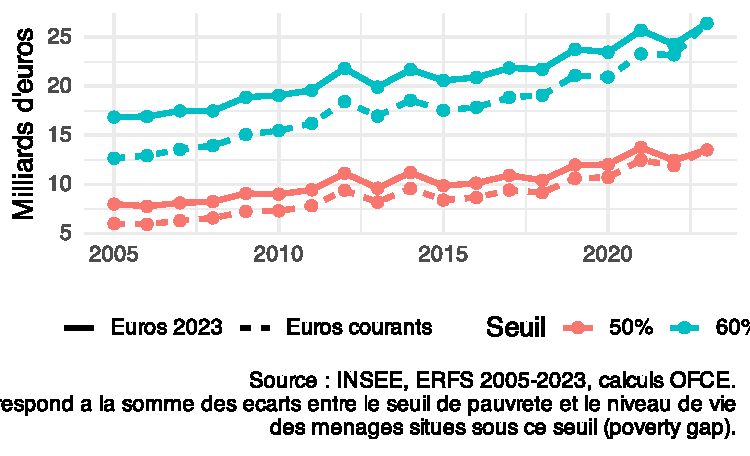
\includegraphics[keepaspectratio]{index_files/mediabag/index_files/figure-pdf/fig-cout-erad-1.pdf}}

}

\end{figure}%

La hausse s'accélère à partir de 2018, résultant de la conjonction de
l'augmentation du nombre de ménages pauvres et du creusement de
l'intensité de la pauvreté. Chaque année d'inaction rend l'éradication
plus coûteuse.

L'intensité de la pauvreté\,--- l'écart relatif moyen entre le niveau de
vie des personnes pauvres et le seuil\,--- se situe autour de 20\,\% au
seuil de 60\,\%, signifiant qu'en moyenne, les personnes pauvres
disposent d'un niveau de vie inférieur de 20\,\% au seuil. Réduire cette
intensité d'un point de pourcentage requiert un transfert de 1\,\% du
seuil à chaque ménage pauvre. Ce coût marginal a augmenté de 40\,\% en
euros constants entre 2005 et 2023, passant de 0,75 à 1,05~milliard
d'euros au seuil de 60\,\% (Graphique~\ref{fig-cout-intensite}).

\begin{figure}

\caption{\label{fig-cout-intensite}Coût de la réduction d'un point
d'intensité de la pauvreté (2005-2023), en milliards d'euros constants
2023, aux seuils de 50\,\% et 60\,\% de la médiane.}

\centering{

\pandocbounded{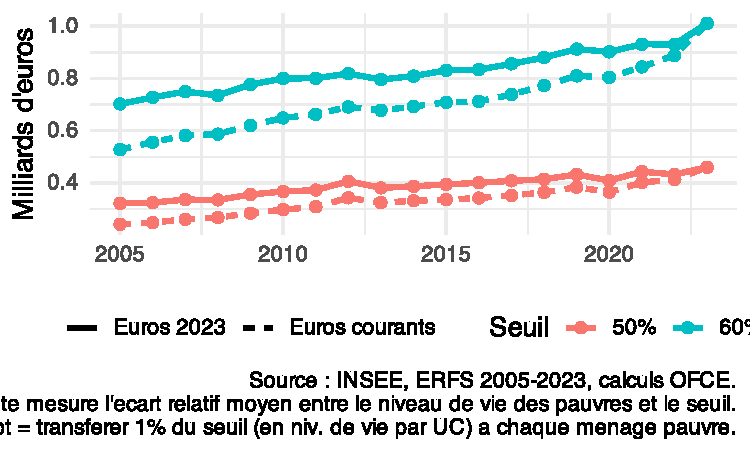
\includegraphics[keepaspectratio]{index_files/mediabag/index_files/figure-pdf/fig-cout-intensite-1.pdf}}

}

\end{figure}%

La progression est quasi linéaire et résulte mécaniquement de la hausse
du seuil et de l'augmentation du nombre de ménages pauvres. Ce résultat
souligne l'intérêt d'une intervention précoce\,: chaque année de report
accroît le coût marginal de la lutte contre la pauvreté.

\section{Au-delà de la pauvreté monétaire\,: le reste à
vivre}\label{au-deluxe0-de-la-pauvretuxe9-monuxe9taire-le-reste-uxe0-vivre}

Le taux de pauvreté monétaire, fondé sur le seul revenu disponible, ne
renseigne pas sur les conditions de vie effectives des ménages. Deux
ménages disposant du même niveau de vie peuvent connaître des réalités
budgétaires très différentes selon le poids de leurs dépenses
incompressibles\,--- logement, alimentation, énergie. L'approche par le
« reste à vivre »\,--- défini ici comme le niveau de vie diminué des
dépenses d'alimentation et de logement\,--- vise à combler cette lacune.
Elle est particulièrement pertinente dans le contexte récent de forte
inflation des prix alimentaires et de l'énergie, qui a affecté de
manière disproportionnée les ménages les plus modestes. Au-delà du
revenu monétaire, l'accès à des services publics de qualité\,---
transports, santé, éducation\,--- constitue un élément décisif des
conditions de vie et de l'égalité des chances (André, 2025).

\begin{tcolorbox}[enhanced jigsaw, leftrule=.75mm, breakable, toptitle=1mm, toprule=.15mm, title={Encadré 6\,--- Imputation de la consommation dans l'ERFS}, opacityback=0, arc=.35mm, opacitybacktitle=0.6, colback=white, coltitle=black, colframe=quarto-callout-note-color-frame, left=2mm, colbacktitle=quarto-callout-note-color!10!white, bottomtitle=1mm, titlerule=0mm, rightrule=.15mm, bottomrule=.15mm]

L'ERFS ne contenant pas d'information sur les dépenses de consommation,
celles-ci sont imputées à partir de l'enquête Budget de Famille (BDF)
2017 de l'INSEE. La procédure se décompose en trois étapes\,:

Étape 1\,--- Calcul des taux de consommation dans BDF. Pour chaque
strate de ménages\,--- définie par le croisement du quintile de niveau
de vie, du type de ménage (5 modalités), de la taille d'unité urbaine (3
modalités) et du statut d'occupation du logement (3 modalités)\,---, on
calcule les taux de consommation par division COICOP (C01 à C12) selon
le ratio des moyennes pondérées\,:

\[tx_{poste,s} = \frac{\sum_{i \in s} C_{poste,i} \times w_i}{\sum_{i \in s} REVDISP_i \times w_i}\]

Cette approche par le ratio des moyennes (plutôt que la moyenne des
ratios) assure la robustesse aux observations à faible revenu
disponible.

Étape 2\,--- Imputation dans l'ERFS. Les mêmes strates sont construites
dans l'ERFS 2018, et les taux BDF sont appariés aux ménages ERFS. Pour
le statut d'occupation du logement, on utilise la variable corrigée
disponible dans l'ERFS (qui corrige les incohérences de déclaration),
plutôt que la variable brute de statut d'occupation (SO). Lorsque la
strate complète (225 cellules) ne permet pas l'appariement\,--- ce qui
concerne notamment l'année 2017 où le statut d'occupation n'est
disponible que pour 21\,\% des ménages\,---, une strate réduite (75
cellules, sans le statut d'occupation) est utilisée en repli.

Étape 3\,--- Indexation temporelle. Pour chaque année \(t\) de 2018 à
2023, les taux de consommation sont appliqués au niveau de vie de chaque
ménage ERFS et indexés sur l'évolution de l'IPC par division COICOP\,:

\[conso_{poste,i,t} = tx_{poste,s(i)} \times nivviem_{i,t} \times \frac{IPC_{poste,t}}{IPC_{poste,2018}}\]

Les dépenses contraintes sont définies comme la somme des postes C01
(produits alimentaires), C02 (boissons alcoolisées, tabac) et C04
(logement, eau, gaz, électricité). Le reste à vivre correspond à\,:
\(RAV_i = nivviem_i - conso\_contrainte_i\).

\end{tcolorbox}

\begin{tcolorbox}[enhanced jigsaw, leftrule=.75mm, breakable, toptitle=1mm, toprule=.15mm, title={Hypothèse de stabilité de la structure de consommation}, opacityback=0, arc=.35mm, opacitybacktitle=0.6, colback=white, coltitle=black, colframe=quarto-callout-warning-color-frame, left=2mm, colbacktitle=quarto-callout-warning-color!10!white, bottomtitle=1mm, titlerule=0mm, rightrule=.15mm, bottomrule=.15mm]

L'ensemble des résultats présentés dans cette section repose sur une
hypothèse forte\,: la stabilité de la structure de consommation des
ménages au cours du temps. Les taux de consommation par poste COICOP,
estimés à partir de BDF 2017, sont supposés constants et seuls les prix
(via l'IPC) et le niveau de vie font varier les montants imputés.

Or, cette hypothèse est mise à l'épreuve par les ajustements observés
lors de la reprise inflationniste de 2021-2023. Les données de la
comptabilité nationale et les enquêtes de conjoncture montrent que les
ménages\,--- et en particulier les plus modestes\,--- ont
significativement modifié leur structure de consommation face à la
hausse des prix (INSEE, 2023b). La consommation alimentaire en volume a
notamment reculé en 2022 et 2023, les ménages arbitrant en faveur de
produits moins chers (\emph{downgrading}), réduisant les quantités
achetées ou renonçant à certains achats. Des comportements similaires
ont été documentés pour les dépenses d'énergie (sobriété énergétique) et
les transports (report modal).

En conséquence, les résultats présentés ici doivent être interprétés
comme des estimations à structure de consommation constante, qui tendent
vraisemblablement à surestimer le poids des dépenses contraintes sur la
période récente, puisqu'ils ne captent pas les ajustements de volume
opérés par les ménages. Ils constituent néanmoins un indicateur
pertinent de la pression inflationniste subie par les différentes
catégories de ménages, indépendamment de leur capacité d'adaptation.

\end{tcolorbox}

Pour les ménages vivant sous le seuil de pauvreté à 60\,\%, les dépenses
d'alimentation et de logement absorbent une part croissante et
considérable du niveau de vie, de l'ordre de 40\,\% sur la période
récente, contre moins de 27\,\% pour les ménages non pauvres
(Graphique~\ref{fig-part-contrainte}). L'écart, déjà substantiel en
début de période, tend à se creuser sous l'effet de la poussée
inflationniste de 2022-2023, les prix alimentaires ayant progressé de
27\,\% entre 2018 et 2023 selon l'IPC (division C01).

\begin{figure}

\caption{\label{fig-part-contrainte}Part des dépenses contraintes
(alimentation et logement) dans le niveau de vie, ménages pauvres et non
pauvres (2018-2023).}

\centering{

\pandocbounded{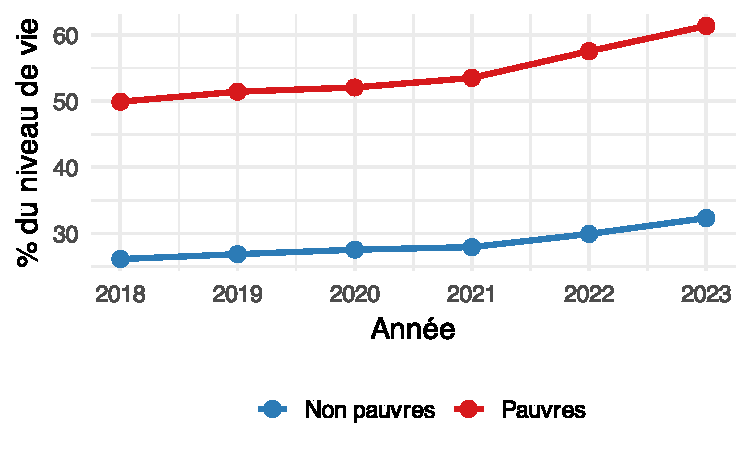
\includegraphics[keepaspectratio]{index_files/mediabag/index_files/figure-pdf/fig-part-contrainte-1.pdf}}

}

\end{figure}%

Le reste à vivre mensuel des ménages pauvres se situe à un niveau
extrêmement contraint\,--- de l'ordre de quelques centaines d'euros par
unité de consommation\,---, ce montant devant couvrir l'ensemble des
autres besoins essentiels\,: transports, santé, habillement, éducation,
loisirs et communications (Graphique~\ref{fig-rav-mensuel}). Pour les
ménages non pauvres, le reste à vivre est nettement plus confortable et
progresse régulièrement. La divergence des trajectoires met en évidence
un phénomène de double peine\,: les ménages modestes subissent une
inflation plus forte sur les postes incompressibles tout en disposant
d'une marge de manœuvre budgétaire initiale considérablement plus
réduite.

\begin{figure}

\caption{\label{fig-rav-mensuel}Reste à vivre mensuel moyen par unité de
consommation, après déduction des dépenses d'alimentation et de
logement, ménages pauvres et non pauvres (2018-2023).}

\centering{

\pandocbounded{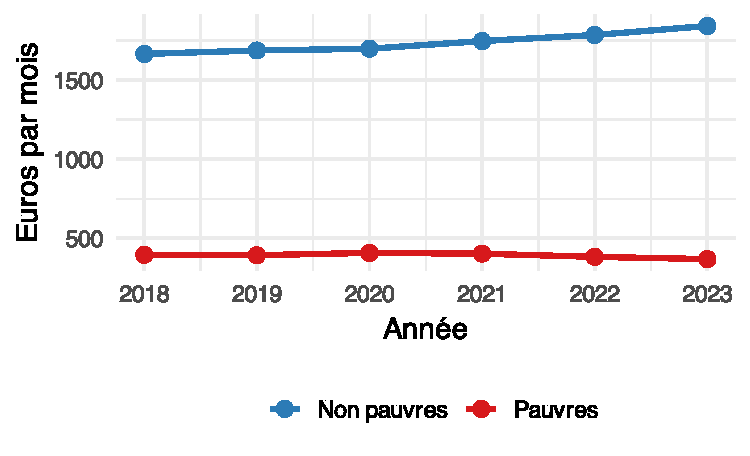
\includegraphics[keepaspectratio]{index_files/mediabag/index_files/figure-pdf/fig-rav-mensuel-1.pdf}}

}

\end{figure}%

L'analyse par grand poste de consommation permet de préciser les
mécanismes à l'œuvre. L'alimentation pèse près de deux fois plus lourd
dans le budget des ménages pauvres que dans celui des ménages non
pauvres, en part du niveau de vie (Graphique~\ref{fig-conso-postes}). Le
logement et l'énergie présentent un différentiel similaire. En revanche,
les postes à caractère plus discrétionnaire\,--- loisirs, restauration,
habillement\,--- sont mécaniquement comprimés chez les ménages pauvres,
traduisant un arbitrage budgétaire sévèrement contraint. L'accélération
des prix alimentaires en 2022-2023 frappe de manière disproportionnée
les ménages les plus modestes, dont la structure de consommation est
fortement concentrée sur ce poste.

\begin{figure}

\caption{\label{fig-conso-postes}Part de chaque grand poste de
consommation dans le niveau de vie (en\,\%), ménages pauvres et non
pauvres (2018-2023).}

\centering{

\pandocbounded{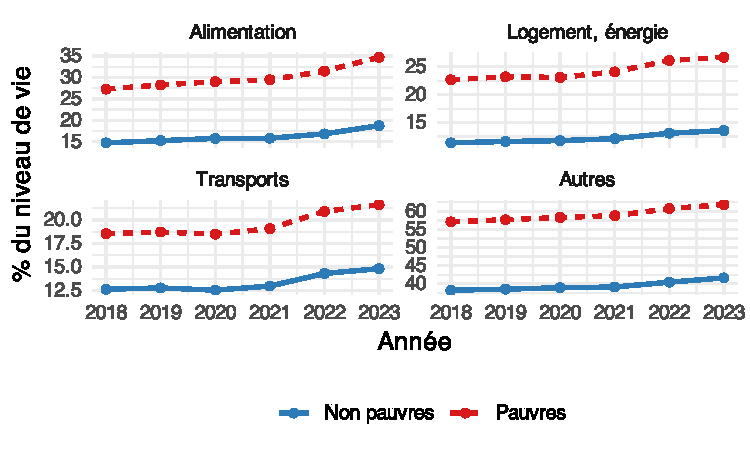
\includegraphics[keepaspectratio]{index_files/mediabag/index_files/figure-pdf/fig-conso-postes-1.pdf}}

}

\end{figure}%

La ventilation par quintile de niveau de vie confirme le gradient social
prononcé des contraintes budgétaires
(Graphique~\ref{fig-quintile-contrainte}). Les 20\,\% des ménages les
plus modestes (premier quintile) consacrent une part nettement
supérieure de leur niveau de vie aux dépenses contraintes par rapport
aux quintiles supérieurs. Ce gradient s'accentue sur la période récente
sous l'effet de la hausse différenciée des prix par poste de
consommation, qui touche proportionnellement davantage les ménages à
faible revenu.

\begin{figure}

\caption{\label{fig-quintile-contrainte}Part des dépenses contraintes
dans le niveau de vie, par quintile de niveau de vie (2018-2023).}

\centering{

\pandocbounded{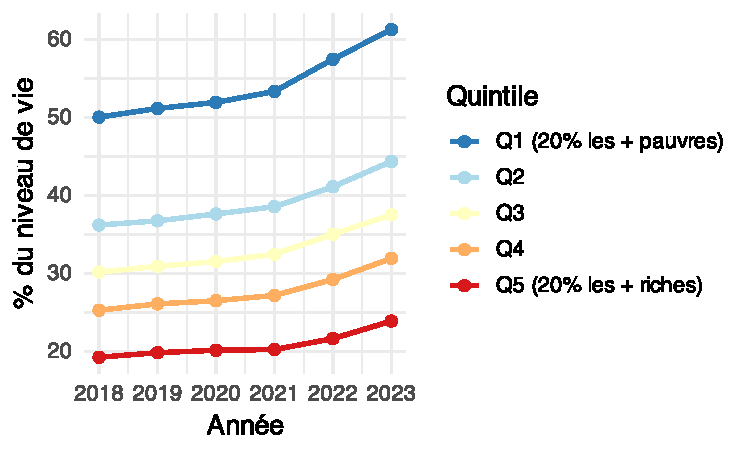
\includegraphics[keepaspectratio]{index_files/mediabag/index_files/figure-pdf/fig-quintile-contrainte-1.pdf}}

}

\end{figure}%

L'ensemble de ces résultats plaide pour une approche de la lutte contre
la pauvreté qui ne se limite pas au seul critère de revenu monétaire
mais intègre la réalité des dépenses contraintes. Plusieurs axes
d'intervention se dessinent\,:

\begin{itemize}
\tightlist
\item
  la revalorisation ciblée des minima sociaux, tenant compte de
  l'inflation effective subie par les ménages modestes\,--- qui s'écarte
  significativement de l'inflation moyenne\,--- plutôt que de la seule
  évolution de l'IPC d'ensemble ((Conseil national des politiques de
  lutte contre la pauvreté et l'exclusion sociale (CNLE), 2025))\,;
\item
  le renforcement des aides au logement, dont l'efficacité s'érode face
  à la progression des loyers et des charges, en particulier
  énergétiques\,;
\item
  le développement de politiques alimentaires visant à atténuer le poids
  du premier poste de dépense des ménages pauvres (chèque alimentaire,
  tarification sociale de la restauration collective) ((Haut Conseil de
  la famille, de l'enfance et de l'âge (HCFEA), 2024c))\,;
\item
  le renforcement des services publics dédiés à la petite enfance (modes
  de garde, école dès le plus jeune âge, aide aux parents)\,: une
  stratégie dont les retombées positives sur le parcours de vie et les
  compétences des futurs adultes sont solidement attestées par la
  recherche.
\item
  la définition d'un « reste à vivre décent » comme indicateur
  complémentaire au seuil de pauvreté monétaire, permettant un ciblage
  plus fin de l'action publique.
\end{itemize}

\begin{center}\rule{0.5\linewidth}{0.5pt}\end{center}

\begin{tcolorbox}[enhanced jigsaw, leftrule=.75mm, breakable, toptitle=1mm, toprule=.15mm, title={Données et sources}, opacityback=0, arc=.35mm, opacitybacktitle=0.6, colback=white, coltitle=black, colframe=quarto-callout-note-color-frame, left=2mm, colbacktitle=quarto-callout-note-color!10!white, bottomtitle=1mm, titlerule=0mm, rightrule=.15mm, bottomrule=.15mm]

Source principale\,: INSEE, Enquête Revenus Fiscaux et Sociaux (ERFS),
2005-2023. Calculs de l'auteur.

Enquête Budget de Famille\,: INSEE, BDF 2017, fichiers MENAGE, DEPMEN et
C05 (consommation détaillée par COICOP).

Indices des prix à la consommation\,: INSEE, Banque de données
macroéconomiques (BDM), indices annuels moyens par division COICOP,
ensemble des ménages, France, base 2015 = 100.

L'ensemble des traitements statistiques est réalisé sous R. Le code
source est disponible sur demande auprès de l'auteur.

\end{tcolorbox}

\subsection*{Références}\label{ruxe9fuxe9rences}
\addcontentsline{toc}{subsection}{Références}

\phantomsection\label{refs}
\begin{CSLReferences}{0}{1}
\bibitem[\citeproctext]{ref-andre_2025}
André M. (2025). {«~Les services publics, acteurs majeurs de la
réduction des inégalités~»}, \emph{Informations sociales}, \emph{213},
p.~105‑117.

\bibitem[\citeproctext]{ref-bonnet2022}
Bonnet C G.B., Solaz A. (2022). {«~Does Part-Time Mothering Help Get a
Job? The Role of Shared Custody in Women's Employment~»}, \emph{Eur J
Popul.}, \emph{213}, p.~885‑913.

\bibitem[\citeproctext]{ref-cnle_plf_2026}
Conseil national des politiques de lutte contre la pauvreté et
l'exclusion sociale (CNLE) (2025).
{«~\href{https://solidarites.gouv.fr/sites/solidarite/files/2025-12/CNLE-note-budget-PLF-2026.pdf}{Analyse
du projet de loi de finances (PLF) pour 2026 : Enjeux de lutte contre la
pauvreté}~»}, Note d\textquotesingle analyse budgétaire, Paris, France,
Ministère des Solidarités, de l'Autonomie et de l'Égalité entre les
femmes et les hommes.

\bibitem[\citeproctext]{ref-dares_travailleurs_pauvres_2022}
DARES (2022). {«~Les travailleurs pauvres en France~»}, \emph{DARES
Analyses}, Direction de l'animation de la recherche, des études et des
statistiques.

\bibitem[\citeproctext]{ref-deschutter_2021}
De Schutter O. (2021). {«~Extreme poverty and human rights~»},
A/HRC/47/36, United Nations Human Rights Council.

\bibitem[\citeproctext]{ref-drees_minima_sociaux_2019}
DREES (2019). {«~Minima sociaux et prestations sociales. Ménages aux
revenus modestes et redistribution~»}, \emph{Collection Panoramas de la
DREES --- Social}, Paris, Direction de la recherche, des études, de
l'évaluation et des statistiques.

\bibitem[\citeproctext]{ref-eurofound_2017}
Eurofound (2017).
\emph{\href{https://www.eurofound.europa.eu/publications/report/2017/in-work-poverty-in-the-eu}{In-Work
Poverty in the EU}}, Publications Office of the European Union,
Luxembourg.

\bibitem[\citeproctext]{ref-eurostat_sespros_2023}
Eurostat (2023).
{«~\href{https://ec.europa.eu/eurostat/statistics-explained/index.php?title=Social_protection_statistics_-_expenditure_and_receipts}{Social
protection statistics --- expenditure and receipts (SESPROS)}~»}, Office
statistique de l'Union européenne.

\bibitem[\citeproctext]{ref-fairlie_2005}
Fairlie R.W. (2005). {«~\href{https://doi.org/10.3233/JEM-2005-0259}{An
Extension of the Blinder-Oaxaca Decomposition Technique to Logit and
Probit Models}~»}, \emph{Journal of Economic and Social Measurement},
\emph{30}, n° 4, p.~305‑316.

\bibitem[\citeproctext]{ref-ofce_2020}
Haut Conseil de la famille, de l'enfance et de l'âge (HCFEA) (2024a).
{«~\href{https://www.egalite-femmes-hommes.gouv.fr/etude-sur-la-situation-economique-et-sociale-des-parents-isoles-0}{Étude
sur la situation économique et sociale des parents isolés}~»}, Rapport
d\textquotesingle étude, Paris, France, Secrétariat d'État chargé de
l'Égalité entre les femmes et les hommes et de la Lutte contre les
discriminations.

\bibitem[\citeproctext]{ref-hcfea_pouvoir_achat_2024}
Haut Conseil de la famille, de l'enfance et de l'âge (HCFEA) (2024b).
{«~\href{https://hcfea.gouv.fr/retour-sur-levolution-du-pouvoir-dachat-des-prestations-familiales-et-de-solidarites}{Retour
sur l'évolution du pouvoir d'achat des prestations familiales et de
solidarités}~»}, Note de synthèse, Paris, France, Haut Conseil de la
famille, de l'enfance et de l'âge.

\bibitem[\citeproctext]{ref-hcfea_restauration_scolaire_2024}
Haut Conseil de la famille, de l'enfance et de l'âge (HCFEA) (2024c).
{«~\href{https://hcfea.gouv.fr/la-restauration-scolaire-un-enjeu-majeur-de-politique-publique}{La
restauration scolaire : un enjeu majeur de politique publique}~»},
Rapport d\textquotesingle étude, Paris, France, Haut Conseil de la
famille, de l'enfance et de l'âge.

\bibitem[\citeproctext]{ref-igas_plan_pauvrete_2017}
IGAS (2017). {«~Évaluation du plan pluriannuel contre la pauvreté et
pour l'inclusion sociale~»}, Rapport IGAS N° 2016-121R, Inspection
générale des affaires sociales.

\bibitem[\citeproctext]{ref-insee_familles_monoparentales_2023}
INSEE (2023a).
{«~\href{https://www.insee.fr/fr/statistiques/7707241}{Tableaux de
l'économie française. Familles}~»}, Institut national de la statistique
et des études économiques.

\bibitem[\citeproctext]{ref-insee_focus_291_2023}
INSEE (2023b). {«~En 2023, les ménages ont maintenu leur consommation
alimentaire en valeur mais l'ont réduite en volume~»}, \emph{INSEE
Focus}, Focus 291, Institut national de la statistique et des études
économiques.

\bibitem[\citeproctext]{ref-insee_france_portrait_social_2024}
INSEE (2024). {«~France, portrait social. Édition 2024~»}, \emph{INSEE
Références}, Paris, Institut national de la statistique et des études
économiques.

\bibitem[\citeproctext]{ref-lelievre_pucci_2025}
Lelièvre M., Pucci M. (2025). {«~Évolutions récentes de la pauvreté~»},
\emph{Informations sociales}, \emph{213}, p.~29‑39.

\bibitem[\citeproctext]{ref-madec_2025}
Madec P. (2025). {«~Quel impact du système redistributif sur la pauvreté
monétaire ?~»}, \emph{Informations sociales}, \emph{213}, p.~69‑77.

\bibitem[\citeproctext]{ref-madec_pucci_2025}
Madec P., Pucci M. (2025).
{«~\href{https://shs.cairn.info/revue-informations-sociales-2025-1}{Nouvelles
formes de pauvreté et redistribution}~»}, \emph{Informations sociales},
\emph{213}, p.~6‑12.

\bibitem[\citeproctext]{ref-oaxaca_1973}
Oaxaca R. (1973). {«~\href{https://doi.org/10.2307/2525981}{Male-Female
Wage Differentials in Urban Labor Markets}~»}, \emph{International
Economic Review}, \emph{14}, n° 3, p.~693‑709.

\bibitem[\citeproctext]{ref-oaxaca_ransom_1999}
Oaxaca R.L., Ransom M.R. (1999).
{«~\href{https://doi.org/10.1162/003465399767923908}{Identification in
Detailed Wage Decompositions}~»}, \emph{The Review of Economics and
Statistics}, \emph{81}, n° 1, p.~154‑157.

\bibitem[\citeproctext]{ref-perivier_2016}
Périvier H. (2016). {«~\href{https://doi.org/10.3917/commu.098.0159}{La
pauvreté au prisme du genre}~»}, \emph{Communications}, \emph{98}, n° 1,
p.~159‑173.

\bibitem[\citeproctext]{ref-ponthieux_2006}
Ponthieux S. (2006). {«~Les travailleurs pauvres en France : une
difficile appréhension, une réalité hétérogène~»}, \emph{Travail et
Emploi}, n° 105, p.~9‑23.

\bibitem[\citeproctext]{ref-ponthieux_2009}
Ponthieux S. (2009).
{«~\href{https://www.insee.fr/fr/statistiques/1380868}{Les travailleurs
pauvres comme catégorie statistique. Difficultés méthodologiques et
exploration d'une notion de pauvreté en revenu d'activité}~»}, dans
\emph{Document de travail}, INSEE.

\bibitem[\citeproctext]{ref-pucci_lelievre_2025}
Pucci M., Lelièvre M., Auzuret C. (2025).
{«~\href{https://solidarites.gouv.fr/sites/solidarite/files/2025-05/Panorama-pauvrete-et-exclusion-entre-2015-et-2022-04-2025.pdf}{Analyse
de l'évolution de la pauvreté et de l'exclusion sociale entre 2015 et
2022}~»}, \emph{Panorama}, Paris, Comité scientifique du Conseil
national des politiques de lutte contre la pauvreté et l'exclusion
sociale (CNLE).

\bibitem[\citeproctext]{ref-yun_2005}
Yun M.-S. (2005). {«~\href{https://doi.org/10.1093/ei/cbi053}{A Simple
Solution to the Identification Problem in Detailed Wage
Decompositions}~»}, \emph{Economic Inquiry}, \emph{43}, n° 4,
p.~766‑772.

\end{CSLReferences}




\end{document}
